
% Default to the notebook output style

    


% Inherit from the specified cell style.




    
\documentclass[11pt]{article}

    
    
    \usepackage[T1]{fontenc}
    % Nicer default font (+ math font) than Computer Modern for most use cases
    \usepackage{mathpazo}

    % Basic figure setup, for now with no caption control since it's done
    % automatically by Pandoc (which extracts ![](path) syntax from Markdown).
    \usepackage{graphicx}
    % We will generate all images so they have a width \maxwidth. This means
    % that they will get their normal width if they fit onto the page, but
    % are scaled down if they would overflow the margins.
    \makeatletter
    \def\maxwidth{\ifdim\Gin@nat@width>\linewidth\linewidth
    \else\Gin@nat@width\fi}
    \makeatother
    \let\Oldincludegraphics\includegraphics
    % Set max figure width to be 80% of text width, for now hardcoded.
    \renewcommand{\includegraphics}[1]{\Oldincludegraphics[width=.8\maxwidth]{#1}}
    % Ensure that by default, figures have no caption (until we provide a
    % proper Figure object with a Caption API and a way to capture that
    % in the conversion process - todo).
    \usepackage{caption}
    \DeclareCaptionLabelFormat{nolabel}{}
    \captionsetup{labelformat=nolabel}

    \usepackage{adjustbox} % Used to constrain images to a maximum size 
    \usepackage{xcolor} % Allow colors to be defined
    \usepackage{enumerate} % Needed for markdown enumerations to work
    \usepackage{geometry} % Used to adjust the document margins
    \usepackage{amsmath} % Equations
    \usepackage{amssymb} % Equations
    \usepackage{textcomp} % defines textquotesingle
    % Hack from http://tex.stackexchange.com/a/47451/13684:
    \AtBeginDocument{%
        \def\PYZsq{\textquotesingle}% Upright quotes in Pygmentized code
    }
    \usepackage{upquote} % Upright quotes for verbatim code
    \usepackage{eurosym} % defines \euro
    \usepackage[mathletters]{ucs} % Extended unicode (utf-8) support
    \usepackage[utf8x]{inputenc} % Allow utf-8 characters in the tex document
    \usepackage{fancyvrb} % verbatim replacement that allows latex
    \usepackage{grffile} % extends the file name processing of package graphics 
                         % to support a larger range 
    % The hyperref package gives us a pdf with properly built
    % internal navigation ('pdf bookmarks' for the table of contents,
    % internal cross-reference links, web links for URLs, etc.)
    \usepackage{hyperref}
    \usepackage{longtable} % longtable support required by pandoc >1.10
    \usepackage{booktabs}  % table support for pandoc > 1.12.2
    \usepackage[inline]{enumitem} % IRkernel/repr support (it uses the enumerate* environment)
    \usepackage[normalem]{ulem} % ulem is needed to support strikethroughs (\sout)
                                % normalem makes italics be italics, not underlines
    

    
    
    % Colors for the hyperref package
    \definecolor{urlcolor}{rgb}{0,.145,.698}
    \definecolor{linkcolor}{rgb}{.71,0.21,0.01}
    \definecolor{citecolor}{rgb}{.12,.54,.11}

    % ANSI colors
    \definecolor{ansi-black}{HTML}{3E424D}
    \definecolor{ansi-black-intense}{HTML}{282C36}
    \definecolor{ansi-red}{HTML}{E75C58}
    \definecolor{ansi-red-intense}{HTML}{B22B31}
    \definecolor{ansi-green}{HTML}{00A250}
    \definecolor{ansi-green-intense}{HTML}{007427}
    \definecolor{ansi-yellow}{HTML}{DDB62B}
    \definecolor{ansi-yellow-intense}{HTML}{B27D12}
    \definecolor{ansi-blue}{HTML}{208FFB}
    \definecolor{ansi-blue-intense}{HTML}{0065CA}
    \definecolor{ansi-magenta}{HTML}{D160C4}
    \definecolor{ansi-magenta-intense}{HTML}{A03196}
    \definecolor{ansi-cyan}{HTML}{60C6C8}
    \definecolor{ansi-cyan-intense}{HTML}{258F8F}
    \definecolor{ansi-white}{HTML}{C5C1B4}
    \definecolor{ansi-white-intense}{HTML}{A1A6B2}

    % commands and environments needed by pandoc snippets
    % extracted from the output of `pandoc -s`
    \providecommand{\tightlist}{%
      \setlength{\itemsep}{0pt}\setlength{\parskip}{0pt}}
    \DefineVerbatimEnvironment{Highlighting}{Verbatim}{commandchars=\\\{\}}
    % Add ',fontsize=\small' for more characters per line
    \newenvironment{Shaded}{}{}
    \newcommand{\KeywordTok}[1]{\textcolor[rgb]{0.00,0.44,0.13}{\textbf{{#1}}}}
    \newcommand{\DataTypeTok}[1]{\textcolor[rgb]{0.56,0.13,0.00}{{#1}}}
    \newcommand{\DecValTok}[1]{\textcolor[rgb]{0.25,0.63,0.44}{{#1}}}
    \newcommand{\BaseNTok}[1]{\textcolor[rgb]{0.25,0.63,0.44}{{#1}}}
    \newcommand{\FloatTok}[1]{\textcolor[rgb]{0.25,0.63,0.44}{{#1}}}
    \newcommand{\CharTok}[1]{\textcolor[rgb]{0.25,0.44,0.63}{{#1}}}
    \newcommand{\StringTok}[1]{\textcolor[rgb]{0.25,0.44,0.63}{{#1}}}
    \newcommand{\CommentTok}[1]{\textcolor[rgb]{0.38,0.63,0.69}{\textit{{#1}}}}
    \newcommand{\OtherTok}[1]{\textcolor[rgb]{0.00,0.44,0.13}{{#1}}}
    \newcommand{\AlertTok}[1]{\textcolor[rgb]{1.00,0.00,0.00}{\textbf{{#1}}}}
    \newcommand{\FunctionTok}[1]{\textcolor[rgb]{0.02,0.16,0.49}{{#1}}}
    \newcommand{\RegionMarkerTok}[1]{{#1}}
    \newcommand{\ErrorTok}[1]{\textcolor[rgb]{1.00,0.00,0.00}{\textbf{{#1}}}}
    \newcommand{\NormalTok}[1]{{#1}}
    
    % Additional commands for more recent versions of Pandoc
    \newcommand{\ConstantTok}[1]{\textcolor[rgb]{0.53,0.00,0.00}{{#1}}}
    \newcommand{\SpecialCharTok}[1]{\textcolor[rgb]{0.25,0.44,0.63}{{#1}}}
    \newcommand{\VerbatimStringTok}[1]{\textcolor[rgb]{0.25,0.44,0.63}{{#1}}}
    \newcommand{\SpecialStringTok}[1]{\textcolor[rgb]{0.73,0.40,0.53}{{#1}}}
    \newcommand{\ImportTok}[1]{{#1}}
    \newcommand{\DocumentationTok}[1]{\textcolor[rgb]{0.73,0.13,0.13}{\textit{{#1}}}}
    \newcommand{\AnnotationTok}[1]{\textcolor[rgb]{0.38,0.63,0.69}{\textbf{\textit{{#1}}}}}
    \newcommand{\CommentVarTok}[1]{\textcolor[rgb]{0.38,0.63,0.69}{\textbf{\textit{{#1}}}}}
    \newcommand{\VariableTok}[1]{\textcolor[rgb]{0.10,0.09,0.49}{{#1}}}
    \newcommand{\ControlFlowTok}[1]{\textcolor[rgb]{0.00,0.44,0.13}{\textbf{{#1}}}}
    \newcommand{\OperatorTok}[1]{\textcolor[rgb]{0.40,0.40,0.40}{{#1}}}
    \newcommand{\BuiltInTok}[1]{{#1}}
    \newcommand{\ExtensionTok}[1]{{#1}}
    \newcommand{\PreprocessorTok}[1]{\textcolor[rgb]{0.74,0.48,0.00}{{#1}}}
    \newcommand{\AttributeTok}[1]{\textcolor[rgb]{0.49,0.56,0.16}{{#1}}}
    \newcommand{\InformationTok}[1]{\textcolor[rgb]{0.38,0.63,0.69}{\textbf{\textit{{#1}}}}}
    \newcommand{\WarningTok}[1]{\textcolor[rgb]{0.38,0.63,0.69}{\textbf{\textit{{#1}}}}}
    
    
    % Define a nice break command that doesn't care if a line doesn't already
    % exist.
    \def\br{\hspace*{\fill} \\* }
    % Math Jax compatability definitions
    \def\gt{>}
    \def\lt{<}
    % Document parameters
    \title{project1\_clustering}
    
    
    

    % Pygments definitions
    
\makeatletter
\def\PY@reset{\let\PY@it=\relax \let\PY@bf=\relax%
    \let\PY@ul=\relax \let\PY@tc=\relax%
    \let\PY@bc=\relax \let\PY@ff=\relax}
\def\PY@tok#1{\csname PY@tok@#1\endcsname}
\def\PY@toks#1+{\ifx\relax#1\empty\else%
    \PY@tok{#1}\expandafter\PY@toks\fi}
\def\PY@do#1{\PY@bc{\PY@tc{\PY@ul{%
    \PY@it{\PY@bf{\PY@ff{#1}}}}}}}
\def\PY#1#2{\PY@reset\PY@toks#1+\relax+\PY@do{#2}}

\expandafter\def\csname PY@tok@w\endcsname{\def\PY@tc##1{\textcolor[rgb]{0.73,0.73,0.73}{##1}}}
\expandafter\def\csname PY@tok@c\endcsname{\let\PY@it=\textit\def\PY@tc##1{\textcolor[rgb]{0.25,0.50,0.50}{##1}}}
\expandafter\def\csname PY@tok@cp\endcsname{\def\PY@tc##1{\textcolor[rgb]{0.74,0.48,0.00}{##1}}}
\expandafter\def\csname PY@tok@k\endcsname{\let\PY@bf=\textbf\def\PY@tc##1{\textcolor[rgb]{0.00,0.50,0.00}{##1}}}
\expandafter\def\csname PY@tok@kp\endcsname{\def\PY@tc##1{\textcolor[rgb]{0.00,0.50,0.00}{##1}}}
\expandafter\def\csname PY@tok@kt\endcsname{\def\PY@tc##1{\textcolor[rgb]{0.69,0.00,0.25}{##1}}}
\expandafter\def\csname PY@tok@o\endcsname{\def\PY@tc##1{\textcolor[rgb]{0.40,0.40,0.40}{##1}}}
\expandafter\def\csname PY@tok@ow\endcsname{\let\PY@bf=\textbf\def\PY@tc##1{\textcolor[rgb]{0.67,0.13,1.00}{##1}}}
\expandafter\def\csname PY@tok@nb\endcsname{\def\PY@tc##1{\textcolor[rgb]{0.00,0.50,0.00}{##1}}}
\expandafter\def\csname PY@tok@nf\endcsname{\def\PY@tc##1{\textcolor[rgb]{0.00,0.00,1.00}{##1}}}
\expandafter\def\csname PY@tok@nc\endcsname{\let\PY@bf=\textbf\def\PY@tc##1{\textcolor[rgb]{0.00,0.00,1.00}{##1}}}
\expandafter\def\csname PY@tok@nn\endcsname{\let\PY@bf=\textbf\def\PY@tc##1{\textcolor[rgb]{0.00,0.00,1.00}{##1}}}
\expandafter\def\csname PY@tok@ne\endcsname{\let\PY@bf=\textbf\def\PY@tc##1{\textcolor[rgb]{0.82,0.25,0.23}{##1}}}
\expandafter\def\csname PY@tok@nv\endcsname{\def\PY@tc##1{\textcolor[rgb]{0.10,0.09,0.49}{##1}}}
\expandafter\def\csname PY@tok@no\endcsname{\def\PY@tc##1{\textcolor[rgb]{0.53,0.00,0.00}{##1}}}
\expandafter\def\csname PY@tok@nl\endcsname{\def\PY@tc##1{\textcolor[rgb]{0.63,0.63,0.00}{##1}}}
\expandafter\def\csname PY@tok@ni\endcsname{\let\PY@bf=\textbf\def\PY@tc##1{\textcolor[rgb]{0.60,0.60,0.60}{##1}}}
\expandafter\def\csname PY@tok@na\endcsname{\def\PY@tc##1{\textcolor[rgb]{0.49,0.56,0.16}{##1}}}
\expandafter\def\csname PY@tok@nt\endcsname{\let\PY@bf=\textbf\def\PY@tc##1{\textcolor[rgb]{0.00,0.50,0.00}{##1}}}
\expandafter\def\csname PY@tok@nd\endcsname{\def\PY@tc##1{\textcolor[rgb]{0.67,0.13,1.00}{##1}}}
\expandafter\def\csname PY@tok@s\endcsname{\def\PY@tc##1{\textcolor[rgb]{0.73,0.13,0.13}{##1}}}
\expandafter\def\csname PY@tok@sd\endcsname{\let\PY@it=\textit\def\PY@tc##1{\textcolor[rgb]{0.73,0.13,0.13}{##1}}}
\expandafter\def\csname PY@tok@si\endcsname{\let\PY@bf=\textbf\def\PY@tc##1{\textcolor[rgb]{0.73,0.40,0.53}{##1}}}
\expandafter\def\csname PY@tok@se\endcsname{\let\PY@bf=\textbf\def\PY@tc##1{\textcolor[rgb]{0.73,0.40,0.13}{##1}}}
\expandafter\def\csname PY@tok@sr\endcsname{\def\PY@tc##1{\textcolor[rgb]{0.73,0.40,0.53}{##1}}}
\expandafter\def\csname PY@tok@ss\endcsname{\def\PY@tc##1{\textcolor[rgb]{0.10,0.09,0.49}{##1}}}
\expandafter\def\csname PY@tok@sx\endcsname{\def\PY@tc##1{\textcolor[rgb]{0.00,0.50,0.00}{##1}}}
\expandafter\def\csname PY@tok@m\endcsname{\def\PY@tc##1{\textcolor[rgb]{0.40,0.40,0.40}{##1}}}
\expandafter\def\csname PY@tok@gh\endcsname{\let\PY@bf=\textbf\def\PY@tc##1{\textcolor[rgb]{0.00,0.00,0.50}{##1}}}
\expandafter\def\csname PY@tok@gu\endcsname{\let\PY@bf=\textbf\def\PY@tc##1{\textcolor[rgb]{0.50,0.00,0.50}{##1}}}
\expandafter\def\csname PY@tok@gd\endcsname{\def\PY@tc##1{\textcolor[rgb]{0.63,0.00,0.00}{##1}}}
\expandafter\def\csname PY@tok@gi\endcsname{\def\PY@tc##1{\textcolor[rgb]{0.00,0.63,0.00}{##1}}}
\expandafter\def\csname PY@tok@gr\endcsname{\def\PY@tc##1{\textcolor[rgb]{1.00,0.00,0.00}{##1}}}
\expandafter\def\csname PY@tok@ge\endcsname{\let\PY@it=\textit}
\expandafter\def\csname PY@tok@gs\endcsname{\let\PY@bf=\textbf}
\expandafter\def\csname PY@tok@gp\endcsname{\let\PY@bf=\textbf\def\PY@tc##1{\textcolor[rgb]{0.00,0.00,0.50}{##1}}}
\expandafter\def\csname PY@tok@go\endcsname{\def\PY@tc##1{\textcolor[rgb]{0.53,0.53,0.53}{##1}}}
\expandafter\def\csname PY@tok@gt\endcsname{\def\PY@tc##1{\textcolor[rgb]{0.00,0.27,0.87}{##1}}}
\expandafter\def\csname PY@tok@err\endcsname{\def\PY@bc##1{\setlength{\fboxsep}{0pt}\fcolorbox[rgb]{1.00,0.00,0.00}{1,1,1}{\strut ##1}}}
\expandafter\def\csname PY@tok@kc\endcsname{\let\PY@bf=\textbf\def\PY@tc##1{\textcolor[rgb]{0.00,0.50,0.00}{##1}}}
\expandafter\def\csname PY@tok@kd\endcsname{\let\PY@bf=\textbf\def\PY@tc##1{\textcolor[rgb]{0.00,0.50,0.00}{##1}}}
\expandafter\def\csname PY@tok@kn\endcsname{\let\PY@bf=\textbf\def\PY@tc##1{\textcolor[rgb]{0.00,0.50,0.00}{##1}}}
\expandafter\def\csname PY@tok@kr\endcsname{\let\PY@bf=\textbf\def\PY@tc##1{\textcolor[rgb]{0.00,0.50,0.00}{##1}}}
\expandafter\def\csname PY@tok@bp\endcsname{\def\PY@tc##1{\textcolor[rgb]{0.00,0.50,0.00}{##1}}}
\expandafter\def\csname PY@tok@fm\endcsname{\def\PY@tc##1{\textcolor[rgb]{0.00,0.00,1.00}{##1}}}
\expandafter\def\csname PY@tok@vc\endcsname{\def\PY@tc##1{\textcolor[rgb]{0.10,0.09,0.49}{##1}}}
\expandafter\def\csname PY@tok@vg\endcsname{\def\PY@tc##1{\textcolor[rgb]{0.10,0.09,0.49}{##1}}}
\expandafter\def\csname PY@tok@vi\endcsname{\def\PY@tc##1{\textcolor[rgb]{0.10,0.09,0.49}{##1}}}
\expandafter\def\csname PY@tok@vm\endcsname{\def\PY@tc##1{\textcolor[rgb]{0.10,0.09,0.49}{##1}}}
\expandafter\def\csname PY@tok@sa\endcsname{\def\PY@tc##1{\textcolor[rgb]{0.73,0.13,0.13}{##1}}}
\expandafter\def\csname PY@tok@sb\endcsname{\def\PY@tc##1{\textcolor[rgb]{0.73,0.13,0.13}{##1}}}
\expandafter\def\csname PY@tok@sc\endcsname{\def\PY@tc##1{\textcolor[rgb]{0.73,0.13,0.13}{##1}}}
\expandafter\def\csname PY@tok@dl\endcsname{\def\PY@tc##1{\textcolor[rgb]{0.73,0.13,0.13}{##1}}}
\expandafter\def\csname PY@tok@s2\endcsname{\def\PY@tc##1{\textcolor[rgb]{0.73,0.13,0.13}{##1}}}
\expandafter\def\csname PY@tok@sh\endcsname{\def\PY@tc##1{\textcolor[rgb]{0.73,0.13,0.13}{##1}}}
\expandafter\def\csname PY@tok@s1\endcsname{\def\PY@tc##1{\textcolor[rgb]{0.73,0.13,0.13}{##1}}}
\expandafter\def\csname PY@tok@mb\endcsname{\def\PY@tc##1{\textcolor[rgb]{0.40,0.40,0.40}{##1}}}
\expandafter\def\csname PY@tok@mf\endcsname{\def\PY@tc##1{\textcolor[rgb]{0.40,0.40,0.40}{##1}}}
\expandafter\def\csname PY@tok@mh\endcsname{\def\PY@tc##1{\textcolor[rgb]{0.40,0.40,0.40}{##1}}}
\expandafter\def\csname PY@tok@mi\endcsname{\def\PY@tc##1{\textcolor[rgb]{0.40,0.40,0.40}{##1}}}
\expandafter\def\csname PY@tok@il\endcsname{\def\PY@tc##1{\textcolor[rgb]{0.40,0.40,0.40}{##1}}}
\expandafter\def\csname PY@tok@mo\endcsname{\def\PY@tc##1{\textcolor[rgb]{0.40,0.40,0.40}{##1}}}
\expandafter\def\csname PY@tok@ch\endcsname{\let\PY@it=\textit\def\PY@tc##1{\textcolor[rgb]{0.25,0.50,0.50}{##1}}}
\expandafter\def\csname PY@tok@cm\endcsname{\let\PY@it=\textit\def\PY@tc##1{\textcolor[rgb]{0.25,0.50,0.50}{##1}}}
\expandafter\def\csname PY@tok@cpf\endcsname{\let\PY@it=\textit\def\PY@tc##1{\textcolor[rgb]{0.25,0.50,0.50}{##1}}}
\expandafter\def\csname PY@tok@c1\endcsname{\let\PY@it=\textit\def\PY@tc##1{\textcolor[rgb]{0.25,0.50,0.50}{##1}}}
\expandafter\def\csname PY@tok@cs\endcsname{\let\PY@it=\textit\def\PY@tc##1{\textcolor[rgb]{0.25,0.50,0.50}{##1}}}

\def\PYZbs{\char`\\}
\def\PYZus{\char`\_}
\def\PYZob{\char`\{}
\def\PYZcb{\char`\}}
\def\PYZca{\char`\^}
\def\PYZam{\char`\&}
\def\PYZlt{\char`\<}
\def\PYZgt{\char`\>}
\def\PYZsh{\char`\#}
\def\PYZpc{\char`\%}
\def\PYZdl{\char`\$}
\def\PYZhy{\char`\-}
\def\PYZsq{\char`\'}
\def\PYZdq{\char`\"}
\def\PYZti{\char`\~}
% for compatibility with earlier versions
\def\PYZat{@}
\def\PYZlb{[}
\def\PYZrb{]}
\makeatother


    % Exact colors from NB
    \definecolor{incolor}{rgb}{0.0, 0.0, 0.5}
    \definecolor{outcolor}{rgb}{0.545, 0.0, 0.0}



    
    % Prevent overflowing lines due to hard-to-break entities
    \sloppy 
    % Setup hyperref package
    \hypersetup{
      breaklinks=true,  % so long urls are correctly broken across lines
      colorlinks=true,
      urlcolor=urlcolor,
      linkcolor=linkcolor,
      citecolor=citecolor,
      }
    % Slightly bigger margins than the latex defaults
    
    \geometry{verbose,tmargin=1in,bmargin=1in,lmargin=1in,rmargin=1in}
    
    

    \begin{document}
    
    
    \maketitle
    
    

    
    \section{Comparison of Clustring
Algorithms}\label{comparison-of-clustring-algorithms}

    When I studying Python, this is a homework for me to analyze the
performance of these two clustering methods on various subsets of our
county-level cancer risk data set in the USA.

In particular, we will compare these two clustering methods in three
areas:

\textbf{Efficiency} - Which method computes clusterings more
efficiently?

\textbf{Automation} - Which method requires less human supervision to
generate reasonable clusterings?

\textbf{Quality} - Which method generates clusterings with less error?

    \textbf{The methods of clustering and related information are showed
below} 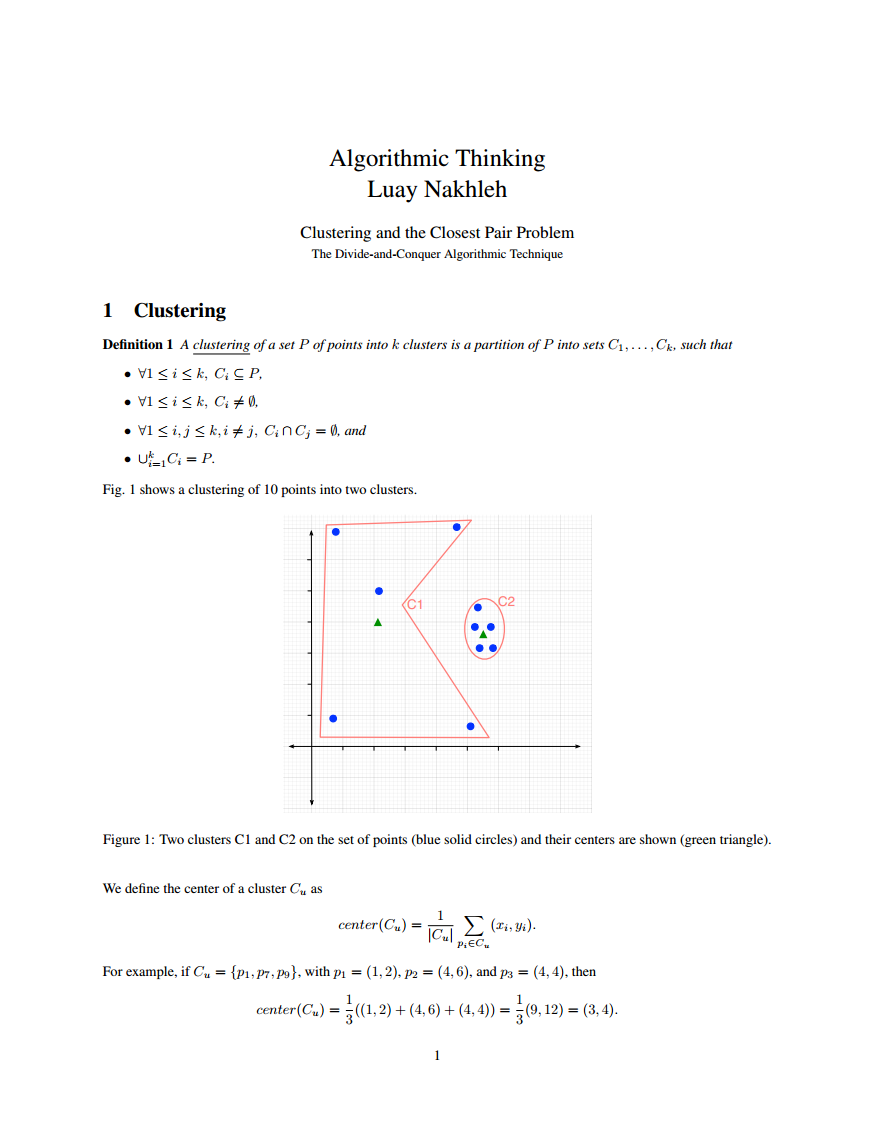
\includegraphics{img/cluster_1.png}
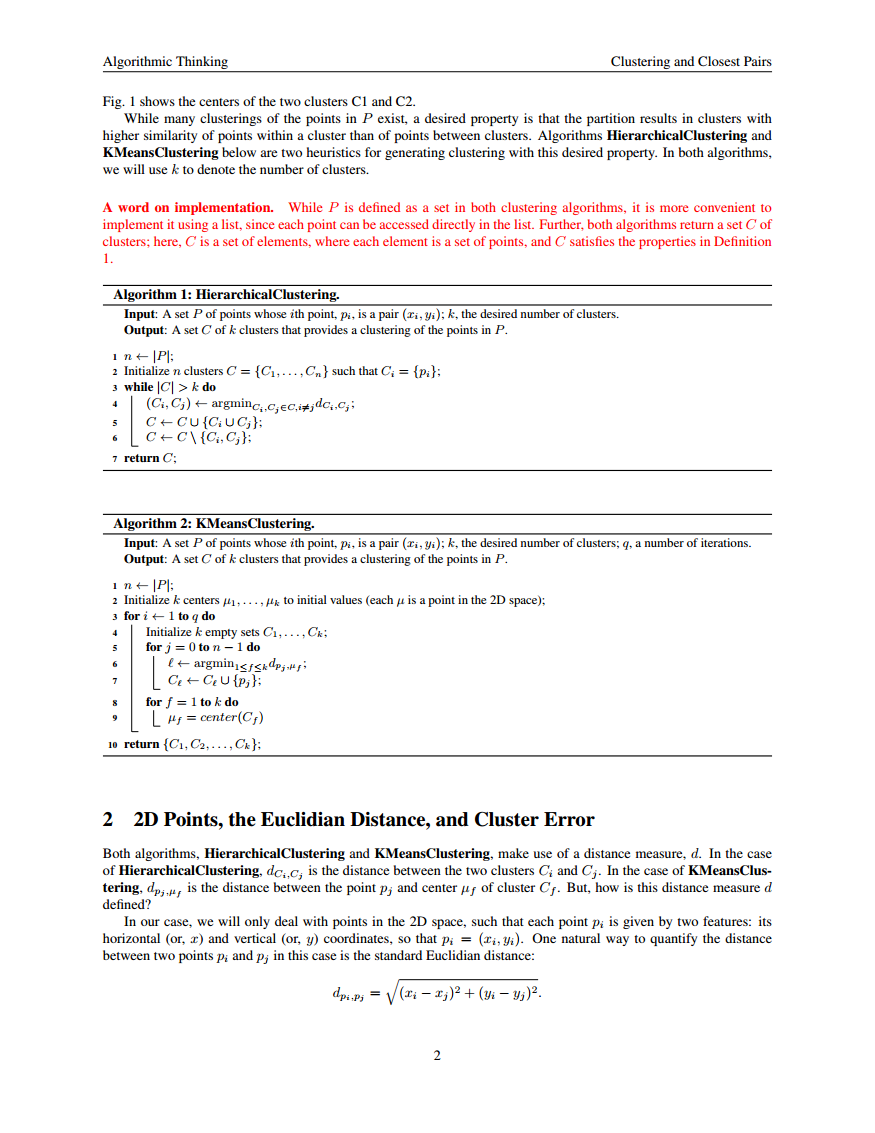
\includegraphics{img/cluster_2.png} 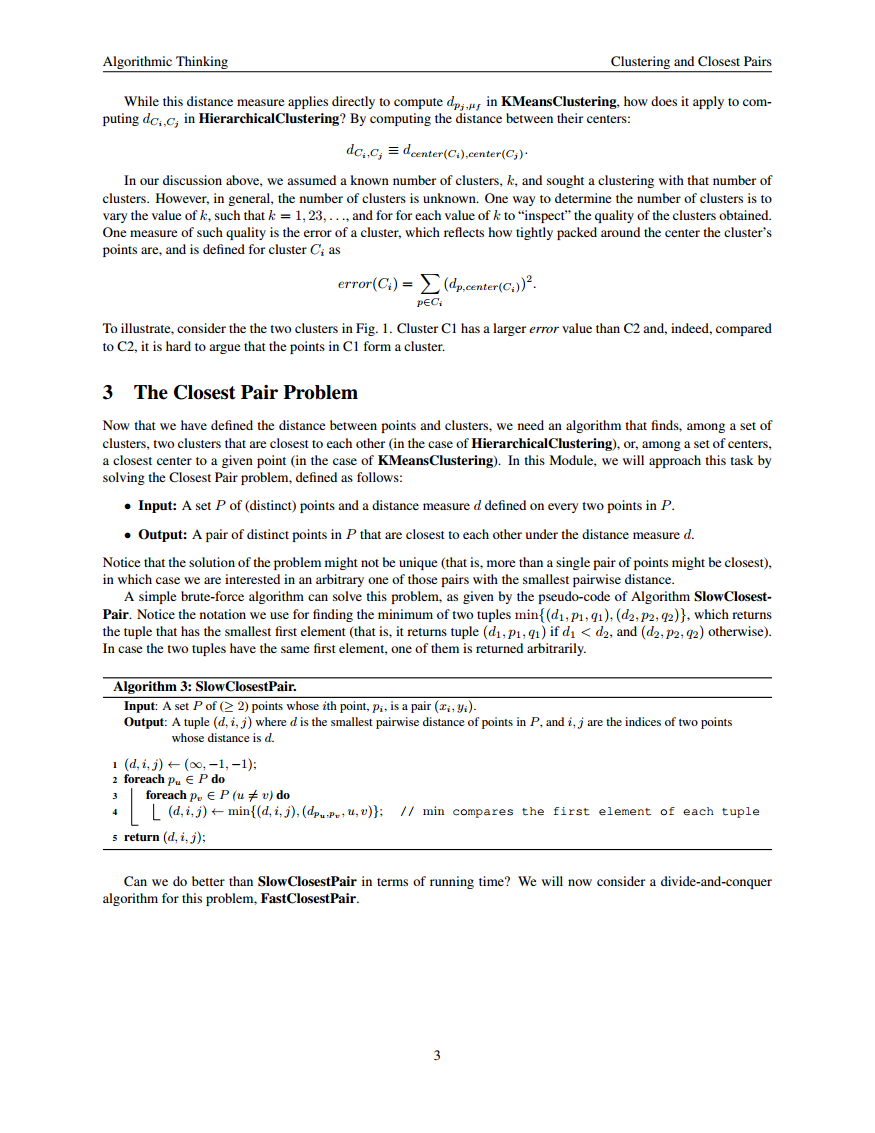
\includegraphics{img/cluster_3.png}
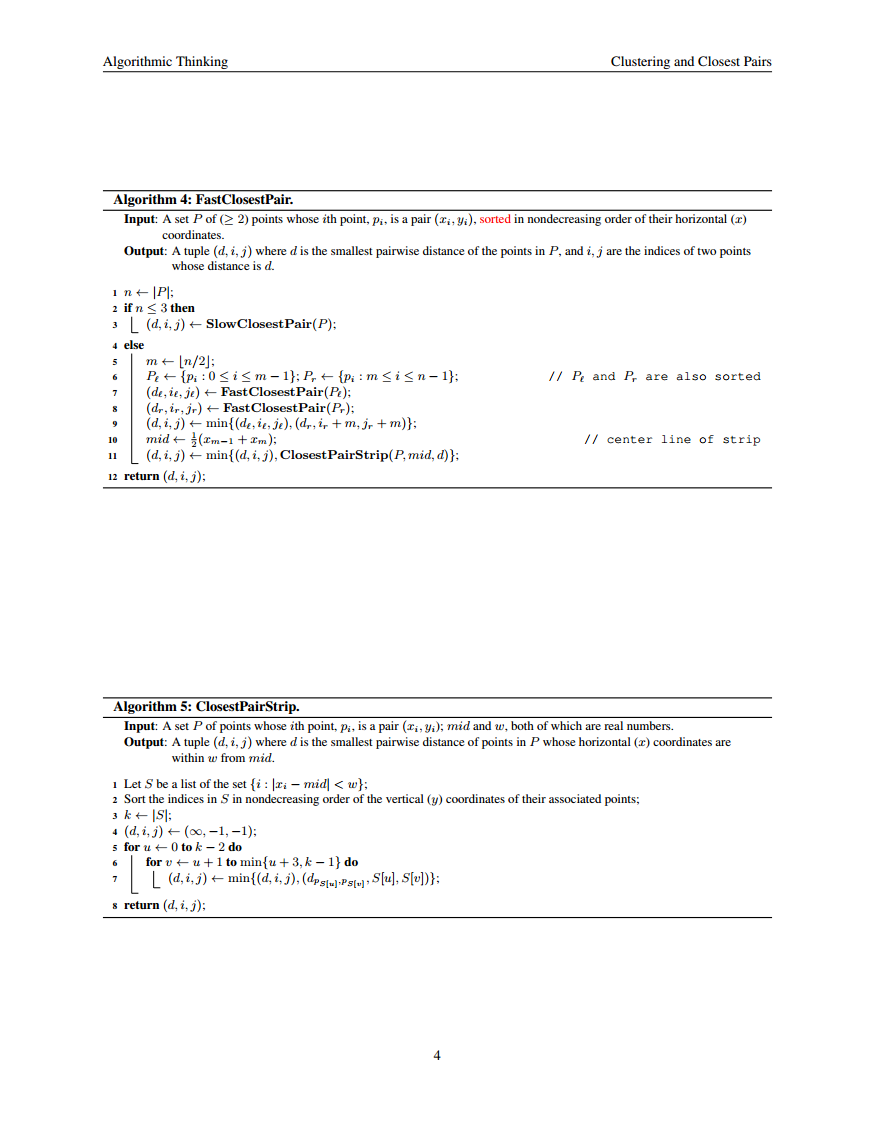
\includegraphics{img/cluster_4.png}

    \textbf{The content below is my answer to this project task.}

    \section{My Work}\label{my-work}

    First, here is a Class Cluster to store the different clusters we
generate.

    \begin{Verbatim}[commandchars=\\\{\}]
{\color{incolor}In [{\color{incolor}4}]:} \PY{l+s+sd}{\PYZdq{}\PYZdq{}\PYZdq{}}
        \PY{l+s+sd}{Cluster class for Module 3}
        \PY{l+s+sd}{\PYZdq{}\PYZdq{}\PYZdq{}}
        
        \PY{k+kn}{import} \PY{n+nn}{math}
        
        
        \PY{k}{class} \PY{n+nc}{Cluster}\PY{p}{:}
            \PY{l+s+sd}{\PYZdq{}\PYZdq{}\PYZdq{}}
        \PY{l+s+sd}{    Class for creating and merging clusters of counties}
        \PY{l+s+sd}{    \PYZdq{}\PYZdq{}\PYZdq{}}
        
            \PY{k}{def} \PY{n+nf}{\PYZus{}\PYZus{}init\PYZus{}\PYZus{}}\PY{p}{(}\PY{n+nb+bp}{self}\PY{p}{,} \PY{n}{fips\PYZus{}codes}\PY{p}{,} \PY{n}{horiz\PYZus{}pos}\PY{p}{,} \PY{n}{vert\PYZus{}pos}\PY{p}{,} \PY{n}{population}\PY{p}{,} \PY{n}{risk}\PY{p}{)}\PY{p}{:}
                \PY{l+s+sd}{\PYZdq{}\PYZdq{}\PYZdq{}}
        \PY{l+s+sd}{        Create a cluster based the models a set of counties\PYZsq{} data}
        \PY{l+s+sd}{        \PYZdq{}\PYZdq{}\PYZdq{}}
                \PY{n+nb+bp}{self}\PY{o}{.}\PY{n}{\PYZus{}fips\PYZus{}codes} \PY{o}{=} \PY{n}{fips\PYZus{}codes}
                \PY{n+nb+bp}{self}\PY{o}{.}\PY{n}{\PYZus{}horiz\PYZus{}center} \PY{o}{=} \PY{n}{horiz\PYZus{}pos}
                \PY{n+nb+bp}{self}\PY{o}{.}\PY{n}{\PYZus{}vert\PYZus{}center} \PY{o}{=} \PY{n}{vert\PYZus{}pos}
                \PY{n+nb+bp}{self}\PY{o}{.}\PY{n}{\PYZus{}total\PYZus{}population} \PY{o}{=} \PY{n}{population}
                \PY{n+nb+bp}{self}\PY{o}{.}\PY{n}{\PYZus{}averaged\PYZus{}risk} \PY{o}{=} \PY{n}{risk}
        
            \PY{k}{def} \PY{n+nf}{\PYZus{}\PYZus{}repr\PYZus{}\PYZus{}}\PY{p}{(}\PY{n+nb+bp}{self}\PY{p}{)}\PY{p}{:}
                \PY{l+s+sd}{\PYZdq{}\PYZdq{}\PYZdq{}}
        \PY{l+s+sd}{        String representation assuming the module is \PYZdq{}alg\PYZus{}cluster\PYZdq{}.}
        \PY{l+s+sd}{        \PYZdq{}\PYZdq{}\PYZdq{}}
                \PY{n}{rep} \PY{o}{=} \PY{l+s+s2}{\PYZdq{}}\PY{l+s+s2}{Cluster(}\PY{l+s+s2}{\PYZdq{}}
                \PY{n}{rep} \PY{o}{+}\PY{o}{=} \PY{n+nb}{str}\PY{p}{(}\PY{n+nb+bp}{self}\PY{o}{.}\PY{n}{\PYZus{}fips\PYZus{}codes}\PY{p}{)} \PY{o}{+} \PY{l+s+s2}{\PYZdq{}}\PY{l+s+s2}{, }\PY{l+s+s2}{\PYZdq{}}
                \PY{n}{rep} \PY{o}{+}\PY{o}{=} \PY{n+nb}{str}\PY{p}{(}\PY{n+nb+bp}{self}\PY{o}{.}\PY{n}{\PYZus{}horiz\PYZus{}center}\PY{p}{)} \PY{o}{+} \PY{l+s+s2}{\PYZdq{}}\PY{l+s+s2}{, }\PY{l+s+s2}{\PYZdq{}}
                \PY{n}{rep} \PY{o}{+}\PY{o}{=} \PY{n+nb}{str}\PY{p}{(}\PY{n+nb+bp}{self}\PY{o}{.}\PY{n}{\PYZus{}vert\PYZus{}center}\PY{p}{)} \PY{o}{+} \PY{l+s+s2}{\PYZdq{}}\PY{l+s+s2}{, }\PY{l+s+s2}{\PYZdq{}}
                \PY{n}{rep} \PY{o}{+}\PY{o}{=} \PY{n+nb}{str}\PY{p}{(}\PY{n+nb+bp}{self}\PY{o}{.}\PY{n}{\PYZus{}total\PYZus{}population}\PY{p}{)} \PY{o}{+} \PY{l+s+s2}{\PYZdq{}}\PY{l+s+s2}{, }\PY{l+s+s2}{\PYZdq{}}
                \PY{n}{rep} \PY{o}{+}\PY{o}{=} \PY{n+nb}{str}\PY{p}{(}\PY{n+nb+bp}{self}\PY{o}{.}\PY{n}{\PYZus{}averaged\PYZus{}risk}\PY{p}{)} \PY{o}{+} \PY{l+s+s2}{\PYZdq{}}\PY{l+s+s2}{)}\PY{l+s+s2}{\PYZdq{}}
                \PY{k}{return} \PY{n}{rep}
        
            \PY{k}{def} \PY{n+nf}{fips\PYZus{}codes}\PY{p}{(}\PY{n+nb+bp}{self}\PY{p}{)}\PY{p}{:}
                \PY{l+s+sd}{\PYZdq{}\PYZdq{}\PYZdq{}}
        \PY{l+s+sd}{        Get the cluster\PYZsq{}s set of FIPS codes}
        \PY{l+s+sd}{        \PYZdq{}\PYZdq{}\PYZdq{}}
                \PY{k}{return} \PY{n+nb+bp}{self}\PY{o}{.}\PY{n}{\PYZus{}fips\PYZus{}codes}
        
            \PY{k}{def} \PY{n+nf}{horiz\PYZus{}center}\PY{p}{(}\PY{n+nb+bp}{self}\PY{p}{)}\PY{p}{:}
                \PY{l+s+sd}{\PYZdq{}\PYZdq{}\PYZdq{}}
        \PY{l+s+sd}{        Get the averged horizontal center of cluster}
        \PY{l+s+sd}{        \PYZdq{}\PYZdq{}\PYZdq{}}
                \PY{k}{return} \PY{n+nb+bp}{self}\PY{o}{.}\PY{n}{\PYZus{}horiz\PYZus{}center}
        
            \PY{k}{def} \PY{n+nf}{vert\PYZus{}center}\PY{p}{(}\PY{n+nb+bp}{self}\PY{p}{)}\PY{p}{:}
                \PY{l+s+sd}{\PYZdq{}\PYZdq{}\PYZdq{}}
        \PY{l+s+sd}{        Get the averaged vertical center of the cluster}
        \PY{l+s+sd}{        \PYZdq{}\PYZdq{}\PYZdq{}}
                \PY{k}{return} \PY{n+nb+bp}{self}\PY{o}{.}\PY{n}{\PYZus{}vert\PYZus{}center}
        
            \PY{k}{def} \PY{n+nf}{total\PYZus{}population}\PY{p}{(}\PY{n+nb+bp}{self}\PY{p}{)}\PY{p}{:}
                \PY{l+s+sd}{\PYZdq{}\PYZdq{}\PYZdq{}}
        \PY{l+s+sd}{        Get the total population for the cluster}
        \PY{l+s+sd}{        \PYZdq{}\PYZdq{}\PYZdq{}}
                \PY{k}{return} \PY{n+nb+bp}{self}\PY{o}{.}\PY{n}{\PYZus{}total\PYZus{}population}
        
            \PY{k}{def} \PY{n+nf}{averaged\PYZus{}risk}\PY{p}{(}\PY{n+nb+bp}{self}\PY{p}{)}\PY{p}{:}
                \PY{l+s+sd}{\PYZdq{}\PYZdq{}\PYZdq{}}
        \PY{l+s+sd}{        Get the averaged risk for the cluster}
        \PY{l+s+sd}{        \PYZdq{}\PYZdq{}\PYZdq{}}
                \PY{k}{return} \PY{n+nb+bp}{self}\PY{o}{.}\PY{n}{\PYZus{}averaged\PYZus{}risk}
        
            \PY{k}{def} \PY{n+nf}{copy}\PY{p}{(}\PY{n+nb+bp}{self}\PY{p}{)}\PY{p}{:}
                \PY{l+s+sd}{\PYZdq{}\PYZdq{}\PYZdq{}}
        \PY{l+s+sd}{        Return a copy of a cluster}
        \PY{l+s+sd}{        \PYZdq{}\PYZdq{}\PYZdq{}}
                \PY{n}{copy\PYZus{}cluster} \PY{o}{=} \PY{n}{Cluster}\PY{p}{(}\PY{n+nb}{set}\PY{p}{(}\PY{n+nb+bp}{self}\PY{o}{.}\PY{n}{\PYZus{}fips\PYZus{}codes}\PY{p}{)}\PY{p}{,} \PY{n+nb+bp}{self}\PY{o}{.}\PY{n}{\PYZus{}horiz\PYZus{}center}\PY{p}{,} \PY{n+nb+bp}{self}\PY{o}{.}\PY{n}{\PYZus{}vert\PYZus{}center}\PY{p}{,}
                                       \PY{n+nb+bp}{self}\PY{o}{.}\PY{n}{\PYZus{}total\PYZus{}population}\PY{p}{,} \PY{n+nb+bp}{self}\PY{o}{.}\PY{n}{\PYZus{}averaged\PYZus{}risk}\PY{p}{)}
                \PY{k}{return} \PY{n}{copy\PYZus{}cluster}
        
            \PY{k}{def} \PY{n+nf}{distance}\PY{p}{(}\PY{n+nb+bp}{self}\PY{p}{,} \PY{n}{other\PYZus{}cluster}\PY{p}{)}\PY{p}{:}
                \PY{l+s+sd}{\PYZdq{}\PYZdq{}\PYZdq{}}
        \PY{l+s+sd}{        Compute the Euclidean distance between two clusters}
        \PY{l+s+sd}{        \PYZdq{}\PYZdq{}\PYZdq{}}
                \PY{n}{vert\PYZus{}dist} \PY{o}{=} \PY{n+nb+bp}{self}\PY{o}{.}\PY{n}{\PYZus{}vert\PYZus{}center} \PY{o}{\PYZhy{}} \PY{n}{other\PYZus{}cluster}\PY{o}{.}\PY{n}{vert\PYZus{}center}\PY{p}{(}\PY{p}{)}
                \PY{n}{horiz\PYZus{}dist} \PY{o}{=} \PY{n+nb+bp}{self}\PY{o}{.}\PY{n}{\PYZus{}horiz\PYZus{}center} \PY{o}{\PYZhy{}} \PY{n}{other\PYZus{}cluster}\PY{o}{.}\PY{n}{horiz\PYZus{}center}\PY{p}{(}\PY{p}{)}
                \PY{k}{return} \PY{n}{math}\PY{o}{.}\PY{n}{sqrt}\PY{p}{(}\PY{n}{vert\PYZus{}dist} \PY{o}{*}\PY{o}{*} \PY{l+m+mi}{2} \PY{o}{+} \PY{n}{horiz\PYZus{}dist} \PY{o}{*}\PY{o}{*} \PY{l+m+mi}{2}\PY{p}{)}
        
            \PY{k}{def} \PY{n+nf}{merge\PYZus{}clusters}\PY{p}{(}\PY{n+nb+bp}{self}\PY{p}{,} \PY{n}{other\PYZus{}cluster}\PY{p}{)}\PY{p}{:}
                \PY{l+s+sd}{\PYZdq{}\PYZdq{}\PYZdq{}}
        \PY{l+s+sd}{        Merge one cluster into another}
        \PY{l+s+sd}{        The merge uses the relatively populations of each}
        \PY{l+s+sd}{        cluster in computing a new center and risk}
        
        \PY{l+s+sd}{        Note that this method mutates self}
        \PY{l+s+sd}{        \PYZdq{}\PYZdq{}\PYZdq{}}
                \PY{k}{if} \PY{n+nb}{len}\PY{p}{(}\PY{n}{other\PYZus{}cluster}\PY{o}{.}\PY{n}{fips\PYZus{}codes}\PY{p}{(}\PY{p}{)}\PY{p}{)} \PY{o}{==} \PY{l+m+mi}{0}\PY{p}{:}
                    \PY{k}{return} \PY{n+nb+bp}{self}
                \PY{k}{else}\PY{p}{:}
                    \PY{n+nb+bp}{self}\PY{o}{.}\PY{n}{\PYZus{}fips\PYZus{}codes}\PY{o}{.}\PY{n}{update}\PY{p}{(}\PY{n+nb}{set}\PY{p}{(}\PY{n}{other\PYZus{}cluster}\PY{o}{.}\PY{n}{fips\PYZus{}codes}\PY{p}{(}\PY{p}{)}\PY{p}{)}\PY{p}{)}
        
                    \PY{c+c1}{\PYZsh{} compute weights for averaging}
                    \PY{n}{self\PYZus{}weight} \PY{o}{=} \PY{n+nb}{float}\PY{p}{(}\PY{n+nb+bp}{self}\PY{o}{.}\PY{n}{\PYZus{}total\PYZus{}population}\PY{p}{)}
                    \PY{n}{other\PYZus{}weight} \PY{o}{=} \PY{n+nb}{float}\PY{p}{(}\PY{n}{other\PYZus{}cluster}\PY{o}{.}\PY{n}{total\PYZus{}population}\PY{p}{(}\PY{p}{)}\PY{p}{)}
                    \PY{n+nb+bp}{self}\PY{o}{.}\PY{n}{\PYZus{}total\PYZus{}population} \PY{o}{=} \PY{n+nb+bp}{self}\PY{o}{.}\PY{n}{\PYZus{}total\PYZus{}population} \PY{o}{+} \PY{n}{other\PYZus{}cluster}\PY{o}{.}\PY{n}{total\PYZus{}population}\PY{p}{(}\PY{p}{)}
                    \PY{n}{self\PYZus{}weight} \PY{o}{/}\PY{o}{=} \PY{n+nb+bp}{self}\PY{o}{.}\PY{n}{\PYZus{}total\PYZus{}population}
                    \PY{n}{other\PYZus{}weight} \PY{o}{/}\PY{o}{=} \PY{n+nb+bp}{self}\PY{o}{.}\PY{n}{\PYZus{}total\PYZus{}population}
        
                    \PY{c+c1}{\PYZsh{} update center and risk using weights}
                    \PY{n+nb+bp}{self}\PY{o}{.}\PY{n}{\PYZus{}vert\PYZus{}center} \PY{o}{=} \PY{n}{self\PYZus{}weight} \PY{o}{*} \PY{n+nb+bp}{self}\PY{o}{.}\PY{n}{\PYZus{}vert\PYZus{}center} \PY{o}{+} \PY{n}{other\PYZus{}weight} \PY{o}{*} \PY{n}{other\PYZus{}cluster}\PY{o}{.}\PY{n}{vert\PYZus{}center}\PY{p}{(}\PY{p}{)}
                    \PY{n+nb+bp}{self}\PY{o}{.}\PY{n}{\PYZus{}horiz\PYZus{}center} \PY{o}{=} \PY{n}{self\PYZus{}weight} \PY{o}{*} \PY{n+nb+bp}{self}\PY{o}{.}\PY{n}{\PYZus{}horiz\PYZus{}center} \PY{o}{+} \PY{n}{other\PYZus{}weight} \PY{o}{*} \PY{n}{other\PYZus{}cluster}\PY{o}{.}\PY{n}{horiz\PYZus{}center}\PY{p}{(}\PY{p}{)}
                    \PY{n+nb+bp}{self}\PY{o}{.}\PY{n}{\PYZus{}averaged\PYZus{}risk} \PY{o}{=} \PY{n}{self\PYZus{}weight} \PY{o}{*} \PY{n+nb+bp}{self}\PY{o}{.}\PY{n}{\PYZus{}averaged\PYZus{}risk} \PY{o}{+} \PY{n}{other\PYZus{}weight} \PY{o}{*} \PY{n}{other\PYZus{}cluster}\PY{o}{.}\PY{n}{averaged\PYZus{}risk}\PY{p}{(}\PY{p}{)}
                    \PY{k}{return} \PY{n+nb+bp}{self}
        
            \PY{k}{def} \PY{n+nf}{cluster\PYZus{}error}\PY{p}{(}\PY{n+nb+bp}{self}\PY{p}{,} \PY{n}{data\PYZus{}table}\PY{p}{)}\PY{p}{:}
                \PY{l+s+sd}{\PYZdq{}\PYZdq{}\PYZdq{}}
        \PY{l+s+sd}{        Input: data\PYZus{}table is the original table of cancer data used in creating the cluster.}
        
        \PY{l+s+sd}{        Output: The error as the sum of the square of the distance from each county}
        \PY{l+s+sd}{        in the cluster to the cluster center (weighted by its population)}
        \PY{l+s+sd}{        \PYZdq{}\PYZdq{}\PYZdq{}}
                \PY{c+c1}{\PYZsh{} Build hash table to accelerate error computation}
                \PY{n}{fips\PYZus{}to\PYZus{}line} \PY{o}{=} \PY{p}{\PYZob{}}\PY{p}{\PYZcb{}}
                \PY{k}{for} \PY{n}{line\PYZus{}idx} \PY{o+ow}{in} \PY{n+nb}{range}\PY{p}{(}\PY{n+nb}{len}\PY{p}{(}\PY{n}{data\PYZus{}table}\PY{p}{)}\PY{p}{)}\PY{p}{:}
                    \PY{n}{line} \PY{o}{=} \PY{n}{data\PYZus{}table}\PY{p}{[}\PY{n}{line\PYZus{}idx}\PY{p}{]}
                    \PY{n}{fips\PYZus{}to\PYZus{}line}\PY{p}{[}\PY{n}{line}\PY{p}{[}\PY{l+m+mi}{0}\PY{p}{]}\PY{p}{]} \PY{o}{=} \PY{n}{line\PYZus{}idx}
        
                \PY{c+c1}{\PYZsh{} compute error as weighted squared distance from counties to cluster center}
                \PY{n}{total\PYZus{}error} \PY{o}{=} \PY{l+m+mi}{0}
                \PY{n}{counties} \PY{o}{=} \PY{n+nb+bp}{self}\PY{o}{.}\PY{n}{fips\PYZus{}codes}\PY{p}{(}\PY{p}{)}
                \PY{k}{for} \PY{n}{county} \PY{o+ow}{in} \PY{n}{counties}\PY{p}{:}
                    \PY{n}{line} \PY{o}{=} \PY{n}{data\PYZus{}table}\PY{p}{[}\PY{n}{fips\PYZus{}to\PYZus{}line}\PY{p}{[}\PY{n}{county}\PY{p}{]}\PY{p}{]}
                    \PY{n}{singleton\PYZus{}cluster} \PY{o}{=} \PY{n}{Cluster}\PY{p}{(}\PY{n+nb}{set}\PY{p}{(}\PY{p}{[}\PY{n}{line}\PY{p}{[}\PY{l+m+mi}{0}\PY{p}{]}\PY{p}{]}\PY{p}{)}\PY{p}{,} \PY{n}{line}\PY{p}{[}\PY{l+m+mi}{1}\PY{p}{]}\PY{p}{,} \PY{n}{line}\PY{p}{[}\PY{l+m+mi}{2}\PY{p}{]}\PY{p}{,} \PY{n}{line}\PY{p}{[}\PY{l+m+mi}{3}\PY{p}{]}\PY{p}{,} \PY{n}{line}\PY{p}{[}\PY{l+m+mi}{4}\PY{p}{]}\PY{p}{)}
                    \PY{n}{singleton\PYZus{}distance} \PY{o}{=} \PY{n+nb+bp}{self}\PY{o}{.}\PY{n}{distance}\PY{p}{(}\PY{n}{singleton\PYZus{}cluster}\PY{p}{)}
                    \PY{n}{total\PYZus{}error} \PY{o}{+}\PY{o}{=} \PY{p}{(}\PY{n}{singleton\PYZus{}distance} \PY{o}{*}\PY{o}{*} \PY{l+m+mi}{2}\PY{p}{)} \PY{o}{*} \PY{n}{singleton\PYZus{}cluster}\PY{o}{.}\PY{n}{total\PYZus{}population}\PY{p}{(}\PY{p}{)}
                \PY{k}{return} \PY{n}{total\PYZus{}error}
\end{Verbatim}


    Then I apply \textbf{2 closest-pair methods} and \textbf{2 clustering
mathod}

    \begin{Verbatim}[commandchars=\\\{\}]
{\color{incolor}In [{\color{incolor}5}]:} \PY{l+s+sd}{\PYZdq{}\PYZdq{}\PYZdq{}}
        \PY{l+s+sd}{We will implement five functions:}
        
        \PY{l+s+sd}{slow\PYZus{}closest\PYZus{}pair(cluster\PYZus{}list)}
        \PY{l+s+sd}{fast\PYZus{}closest\PYZus{}pair(cluster\PYZus{}list)}
        \PY{l+s+sd}{closest\PYZus{}pair\PYZus{}strip(cluster\PYZus{}list, horiz\PYZus{}center, half\PYZus{}width)}
        \PY{l+s+sd}{hierarchical\PYZus{}clustering(cluster\PYZus{}list, num\PYZus{}clusters)}
        \PY{l+s+sd}{kmeans\PYZus{}clustering(cluster\PYZus{}list, num\PYZus{}clusters, num\PYZus{}iterations)}
        
        \PY{l+s+sd}{where cluster\PYZus{}list is a 2D list of clusters in the plane}
        \PY{l+s+sd}{\PYZdq{}\PYZdq{}\PYZdq{}}
        
        
        \PY{c+c1}{\PYZsh{}\PYZsh{}\PYZsh{}\PYZsh{}\PYZsh{}\PYZsh{}\PYZsh{}\PYZsh{}\PYZsh{}\PYZsh{}\PYZsh{}\PYZsh{}\PYZsh{}\PYZsh{}\PYZsh{}\PYZsh{}\PYZsh{}\PYZsh{}\PYZsh{}\PYZsh{}\PYZsh{}\PYZsh{}\PYZsh{}\PYZsh{}\PYZsh{}\PYZsh{}\PYZsh{}\PYZsh{}\PYZsh{}\PYZsh{}\PYZsh{}\PYZsh{}\PYZsh{}\PYZsh{}\PYZsh{}\PYZsh{}\PYZsh{}\PYZsh{}\PYZsh{}\PYZsh{}\PYZsh{}\PYZsh{}\PYZsh{}\PYZsh{}\PYZsh{}\PYZsh{}\PYZsh{}\PYZsh{}\PYZsh{}\PYZsh{}\PYZsh{}\PYZsh{}\PYZsh{}\PYZsh{}}
        \PY{c+c1}{\PYZsh{} Code for closest pairs of clusters}
        
        \PY{k}{def} \PY{n+nf}{min\PYZus{}pair}\PY{p}{(}\PY{n}{pair\PYZus{}a}\PY{p}{,} \PY{n}{pair\PYZus{}b}\PY{p}{)}\PY{p}{:}
            \PY{l+s+sd}{\PYZdq{}\PYZdq{}\PYZdq{}}
        \PY{l+s+sd}{    get the min distance pair}
        \PY{l+s+sd}{    \PYZdq{}\PYZdq{}\PYZdq{}}
            \PY{k}{if} \PY{n}{pair\PYZus{}a}\PY{p}{[}\PY{l+m+mi}{0}\PY{p}{]} \PY{o}{\PYZlt{}}\PY{o}{=} \PY{n}{pair\PYZus{}b}\PY{p}{[}\PY{l+m+mi}{0}\PY{p}{]}\PY{p}{:}
                \PY{k}{return} \PY{n}{pair\PYZus{}a}
            \PY{k}{return} \PY{n}{pair\PYZus{}b}
        
        
        \PY{k}{def} \PY{n+nf}{slow\PYZus{}closest\PYZus{}pair}\PY{p}{(}\PY{n}{cluster\PYZus{}list}\PY{p}{)}\PY{p}{:}
            \PY{l+s+sd}{\PYZdq{}\PYZdq{}\PYZdq{}}
        \PY{l+s+sd}{    Compute the distance between the closest pair of clusters in a list (slow)}
        
        \PY{l+s+sd}{    Input: cluster\PYZus{}list is the list of clusters}
        
        \PY{l+s+sd}{    Output: tuple of the form (dist, idx1, idx2) where the centers of the clusters}
        \PY{l+s+sd}{    cluster\PYZus{}list[idx1] and cluster\PYZus{}list[idx2] have minimum distance dist.}
        \PY{l+s+sd}{    \PYZdq{}\PYZdq{}\PYZdq{}}
            \PY{n}{min\PYZus{}dis} \PY{o}{=} \PY{n+nb}{float}\PY{p}{(}\PY{l+s+s1}{\PYZsq{}}\PY{l+s+s1}{inf}\PY{l+s+s1}{\PYZsq{}}\PY{p}{)}
            \PY{n}{closest\PYZus{}pair} \PY{o}{=} \PY{p}{(}\PY{n}{min\PYZus{}dis}\PY{p}{,} \PY{l+m+mi}{0}\PY{p}{,} \PY{l+m+mi}{0}\PY{p}{)}
            \PY{k}{for} \PY{n}{cluster} \PY{o+ow}{in} \PY{n}{cluster\PYZus{}list}\PY{p}{:}
                \PY{n}{index\PYZus{}c} \PY{o}{=} \PY{n}{cluster\PYZus{}list}\PY{o}{.}\PY{n}{index}\PY{p}{(}\PY{n}{cluster}\PY{p}{)}
                \PY{k}{for} \PY{n}{other\PYZus{}cluster} \PY{o+ow}{in} \PY{n}{cluster\PYZus{}list}\PY{p}{[}\PY{n}{cluster\PYZus{}list}\PY{o}{.}\PY{n}{index}\PY{p}{(}\PY{n}{cluster}\PY{p}{)} \PY{o}{+} \PY{l+m+mi}{1}\PY{p}{:}\PY{p}{]}\PY{p}{:}
                    \PY{n}{dis} \PY{o}{=} \PY{n}{cluster}\PY{o}{.}\PY{n}{distance}\PY{p}{(}\PY{n}{other\PYZus{}cluster}\PY{p}{)}
                    \PY{k}{if} \PY{n}{dis} \PY{o}{\PYZlt{}} \PY{n}{closest\PYZus{}pair}\PY{p}{[}\PY{l+m+mi}{0}\PY{p}{]}\PY{p}{:}
                        \PY{n}{closest\PYZus{}pair} \PY{o}{=} \PY{p}{(}\PY{n}{dis}\PY{p}{,} \PY{n}{index\PYZus{}c}\PY{p}{,} \PY{n}{cluster\PYZus{}list}\PY{o}{.}\PY{n}{index}\PY{p}{(}\PY{n}{other\PYZus{}cluster}\PY{p}{)}\PY{p}{)}
        
            \PY{k}{return} \PY{n}{closest\PYZus{}pair}
        
        
        \PY{k}{def} \PY{n+nf}{closest\PYZus{}pair\PYZus{}strip}\PY{p}{(}\PY{n}{cluster\PYZus{}list}\PY{p}{,} \PY{n}{horiz\PYZus{}center}\PY{p}{,} \PY{n}{half\PYZus{}width}\PY{p}{)}\PY{p}{:}
            \PY{l+s+sd}{\PYZdq{}\PYZdq{}\PYZdq{}}
        \PY{l+s+sd}{    Helper function to compute the closest pair of clusters in a vertical strip}
        
        \PY{l+s+sd}{    Input: cluster\PYZus{}list is a list of clusters produced by fast\PYZus{}closest\PYZus{}pair}
        \PY{l+s+sd}{    horiz\PYZus{}center is the horizontal position of the strip\PYZsq{}s vertical center line}
        \PY{l+s+sd}{    half\PYZus{}width is the half the width of the strip (i.e; the maximum horizontal distance}
        \PY{l+s+sd}{    that a cluster can lie from the center line)}
        
        \PY{l+s+sd}{    Output: tuple of the form (dist, idx1, idx2) where the centers of the clusters}
        \PY{l+s+sd}{    cluster\PYZus{}list[idx1] and cluster\PYZus{}list[idx2] lie in the strip and have minimum distance dist.}
        \PY{l+s+sd}{    \PYZdq{}\PYZdq{}\PYZdq{}}
            \PY{c+c1}{\PYZsh{} don\PYZsq{}t go out of [horiz\PYZus{}l, horiz\PYZus{}r]}
            \PY{n}{cluster\PYZus{}list\PYZus{}m} \PY{o}{=} \PY{p}{[}\PY{p}{]}
            \PY{n}{horiz\PYZus{}l} \PY{o}{=} \PY{n+nb}{max}\PY{p}{(}\PY{n}{cluster\PYZus{}list}\PY{p}{[}\PY{l+m+mi}{0}\PY{p}{]}\PY{o}{.}\PY{n}{horiz\PYZus{}center}\PY{p}{(}\PY{p}{)}\PY{p}{,} \PY{n}{horiz\PYZus{}center} \PY{o}{\PYZhy{}} \PY{n}{half\PYZus{}width}\PY{p}{)}
            \PY{n}{horiz\PYZus{}r} \PY{o}{=} \PY{n+nb}{min}\PY{p}{(}\PY{n}{cluster\PYZus{}list}\PY{p}{[}\PY{o}{\PYZhy{}}\PY{l+m+mi}{1}\PY{p}{]}\PY{o}{.}\PY{n}{horiz\PYZus{}center}\PY{p}{(}\PY{p}{)}\PY{p}{,} \PY{n}{horiz\PYZus{}center} \PY{o}{+} \PY{n}{half\PYZus{}width}\PY{p}{)}
            \PY{c+c1}{\PYZsh{} horiz\PYZus{}l = horiz\PYZus{}center \PYZhy{} half\PYZus{}width}
            \PY{c+c1}{\PYZsh{} horiz\PYZus{}r = horiz\PYZus{}center + half\PYZus{}width}
            \PY{k}{for} \PY{n}{cluster} \PY{o+ow}{in} \PY{n}{cluster\PYZus{}list}\PY{p}{:}
                \PY{k}{if} \PY{n}{horiz\PYZus{}l} \PY{o}{\PYZlt{}}\PY{o}{=} \PY{n}{cluster}\PY{o}{.}\PY{n}{horiz\PYZus{}center}\PY{p}{(}\PY{p}{)} \PY{o}{\PYZlt{}}\PY{o}{=} \PY{n}{horiz\PYZus{}r}\PY{p}{:}
                    \PY{n}{cluster\PYZus{}list\PYZus{}m}\PY{o}{.}\PY{n}{append}\PY{p}{(}\PY{n}{cluster}\PY{p}{)}
        
            \PY{n}{closest\PYZus{}pair} \PY{o}{=} \PY{p}{(}\PY{n+nb}{float}\PY{p}{(}\PY{l+s+s1}{\PYZsq{}}\PY{l+s+s1}{inf}\PY{l+s+s1}{\PYZsq{}}\PY{p}{)}\PY{p}{,} \PY{o}{\PYZhy{}}\PY{l+m+mi}{1}\PY{p}{,} \PY{o}{\PYZhy{}}\PY{l+m+mi}{1}\PY{p}{)}
            \PY{n}{cluster\PYZus{}list\PYZus{}m}\PY{o}{.}\PY{n}{sort}\PY{p}{(}\PY{n}{key}\PY{o}{=}\PY{k}{lambda} \PY{n}{clstr}\PY{p}{:} \PY{n}{clstr}\PY{o}{.}\PY{n}{vert\PYZus{}center}\PY{p}{(}\PY{p}{)}\PY{p}{)}
            \PY{n}{lenth} \PY{o}{=} \PY{n+nb}{len}\PY{p}{(}\PY{n}{cluster\PYZus{}list\PYZus{}m}\PY{p}{)}
            \PY{k}{for} \PY{n}{index\PYZus{}i} \PY{o+ow}{in} \PY{n+nb}{range}\PY{p}{(}\PY{n}{lenth} \PY{o}{\PYZhy{}} \PY{l+m+mi}{1}\PY{p}{)}\PY{p}{:}
                \PY{k}{for} \PY{n}{index\PYZus{}j} \PY{o+ow}{in} \PY{n+nb}{range}\PY{p}{(}\PY{n}{index\PYZus{}i} \PY{o}{+} \PY{l+m+mi}{1}\PY{p}{,} \PY{n+nb}{min}\PY{p}{(}\PY{n}{index\PYZus{}i} \PY{o}{+} \PY{l+m+mi}{4}\PY{p}{,} \PY{n}{lenth}\PY{p}{)}\PY{p}{)}\PY{p}{:}
                    \PY{n}{dis} \PY{o}{=} \PY{n}{cluster\PYZus{}list\PYZus{}m}\PY{p}{[}\PY{n}{index\PYZus{}i}\PY{p}{]}\PY{o}{.}\PY{n}{distance}\PY{p}{(}\PY{n}{cluster\PYZus{}list\PYZus{}m}\PY{p}{[}\PY{n}{index\PYZus{}j}\PY{p}{]}\PY{p}{)}
                    \PY{n}{real\PYZus{}index\PYZus{}i} \PY{o}{=} \PY{n}{cluster\PYZus{}list}\PY{o}{.}\PY{n}{index}\PY{p}{(}\PY{n}{cluster\PYZus{}list\PYZus{}m}\PY{p}{[}\PY{n}{index\PYZus{}i}\PY{p}{]}\PY{p}{)}
                    \PY{n}{real\PYZus{}index\PYZus{}j} \PY{o}{=} \PY{n}{cluster\PYZus{}list}\PY{o}{.}\PY{n}{index}\PY{p}{(}\PY{n}{cluster\PYZus{}list\PYZus{}m}\PY{p}{[}\PY{n}{index\PYZus{}j}\PY{p}{]}\PY{p}{)}
                    \PY{n}{closest\PYZus{}pair} \PY{o}{=} \PY{n}{min\PYZus{}pair}\PY{p}{(}\PY{n}{closest\PYZus{}pair}\PY{p}{,} \PY{p}{(}\PY{n}{dis}\PY{p}{,} \PY{n+nb}{min}\PY{p}{(}\PY{n}{real\PYZus{}index\PYZus{}i}\PY{p}{,} \PY{n}{real\PYZus{}index\PYZus{}j}\PY{p}{)}\PY{p}{,}
                                                           \PY{n+nb}{max}\PY{p}{(}\PY{n}{real\PYZus{}index\PYZus{}i}\PY{p}{,} \PY{n}{real\PYZus{}index\PYZus{}j}\PY{p}{)}\PY{p}{)}\PY{p}{)}
        
            \PY{k}{return} \PY{n}{closest\PYZus{}pair}
        
        
        \PY{k}{def} \PY{n+nf}{fast\PYZus{}closest\PYZus{}pair}\PY{p}{(}\PY{n}{cluster\PYZus{}list}\PY{p}{)}\PY{p}{:}
            \PY{l+s+sd}{\PYZdq{}\PYZdq{}\PYZdq{}}
        \PY{l+s+sd}{    Compute the distance between the closest pair of clusters in a list (fast)}
        
        \PY{l+s+sd}{    Input: cluster\PYZus{}list is list of clusters SORTED such that horizontal positions of their}
        \PY{l+s+sd}{    centers are in ascending order}
        
        \PY{l+s+sd}{    Output: tuple of the form (dist, idx1, idx2) where the centers of the clusters}
        \PY{l+s+sd}{    cluster\PYZus{}list[idx1] and cluster\PYZus{}list[idx2] have minimum distance dist.}
        \PY{l+s+sd}{    \PYZdq{}\PYZdq{}\PYZdq{}}
            \PY{c+c1}{\PYZsh{} print(cluster\PYZus{}list)}
            \PY{k}{if} \PY{n+nb}{len}\PY{p}{(}\PY{n}{cluster\PYZus{}list}\PY{p}{)} \PY{o}{\PYZlt{}} \PY{l+m+mi}{2}\PY{p}{:}
                \PY{k}{return} \PY{n+nb}{float}\PY{p}{(}\PY{l+s+s1}{\PYZsq{}}\PY{l+s+s1}{inf}\PY{l+s+s1}{\PYZsq{}}\PY{p}{)}\PY{p}{,} \PY{o}{\PYZhy{}}\PY{l+m+mi}{1}\PY{p}{,} \PY{o}{\PYZhy{}}\PY{l+m+mi}{1}
            \PY{k}{if} \PY{n+nb}{len}\PY{p}{(}\PY{n}{cluster\PYZus{}list}\PY{p}{)} \PY{o}{==} \PY{l+m+mi}{2}\PY{p}{:}
                \PY{k}{return} \PY{n}{cluster\PYZus{}list}\PY{p}{[}\PY{l+m+mi}{0}\PY{p}{]}\PY{o}{.}\PY{n}{distance}\PY{p}{(}\PY{n}{cluster\PYZus{}list}\PY{p}{[}\PY{l+m+mi}{1}\PY{p}{]}\PY{p}{)}\PY{p}{,} \PY{l+m+mi}{0}\PY{p}{,} \PY{l+m+mi}{1}
        
            \PY{n}{mid\PYZus{}num} \PY{o}{=} \PY{n+nb}{len}\PY{p}{(}\PY{n}{cluster\PYZus{}list}\PY{p}{)} \PY{o}{/}\PY{o}{/} \PY{l+m+mi}{2}
            \PY{n}{closest\PYZus{}pair\PYZus{}l} \PY{o}{=} \PY{n}{fast\PYZus{}closest\PYZus{}pair}\PY{p}{(}\PY{n}{cluster\PYZus{}list}\PY{p}{[}\PY{p}{:}\PY{n}{mid\PYZus{}num}\PY{p}{]}\PY{p}{)}
            \PY{n}{closest\PYZus{}pair\PYZus{}r} \PY{o}{=} \PY{n}{fast\PYZus{}closest\PYZus{}pair}\PY{p}{(}\PY{n}{cluster\PYZus{}list}\PY{p}{[}\PY{n}{mid\PYZus{}num}\PY{p}{:}\PY{p}{]}\PY{p}{)}
            \PY{n}{closest\PYZus{}pair\PYZus{}r} \PY{o}{=} \PY{p}{(}\PY{n}{closest\PYZus{}pair\PYZus{}r}\PY{p}{[}\PY{l+m+mi}{0}\PY{p}{]}\PY{p}{,} \PY{n}{closest\PYZus{}pair\PYZus{}r}\PY{p}{[}\PY{l+m+mi}{1}\PY{p}{]} \PY{o}{+} \PY{n}{mid\PYZus{}num}\PY{p}{,} \PY{n}{closest\PYZus{}pair\PYZus{}r}\PY{p}{[}\PY{l+m+mi}{2}\PY{p}{]} \PY{o}{+} \PY{n}{mid\PYZus{}num}\PY{p}{)}
            \PY{n}{closest\PYZus{}pair} \PY{o}{=} \PY{n}{min\PYZus{}pair}\PY{p}{(}\PY{n}{closest\PYZus{}pair\PYZus{}l}\PY{p}{,} \PY{n}{closest\PYZus{}pair\PYZus{}r}\PY{p}{)}
        
            \PY{n}{mid\PYZus{}horiz} \PY{o}{=} \PY{p}{(}\PY{n}{cluster\PYZus{}list}\PY{p}{[}\PY{n}{mid\PYZus{}num} \PY{o}{\PYZhy{}} \PY{l+m+mi}{1}\PY{p}{]}\PY{o}{.}\PY{n}{horiz\PYZus{}center}\PY{p}{(}\PY{p}{)} \PY{o}{+} \PY{n}{cluster\PYZus{}list}\PY{p}{[}\PY{n}{mid\PYZus{}num}\PY{p}{]}\PY{o}{.}\PY{n}{horiz\PYZus{}center}\PY{p}{(}\PY{p}{)}\PY{p}{)} \PY{o}{/} \PY{l+m+mi}{2}
            \PY{n}{closest\PYZus{}pair} \PY{o}{=} \PY{n}{min\PYZus{}pair}\PY{p}{(}\PY{n}{closest\PYZus{}pair}\PY{p}{,} \PY{n}{closest\PYZus{}pair\PYZus{}strip}\PY{p}{(}\PY{n}{cluster\PYZus{}list}\PY{p}{,} \PY{n}{mid\PYZus{}horiz}\PY{p}{,} \PY{n}{closest\PYZus{}pair}\PY{p}{[}\PY{l+m+mi}{0}\PY{p}{]}\PY{p}{)}\PY{p}{)}
        
            \PY{k}{return} \PY{n}{closest\PYZus{}pair}
        
        
        \PY{c+c1}{\PYZsh{}\PYZsh{}\PYZsh{}\PYZsh{}\PYZsh{}\PYZsh{}\PYZsh{}\PYZsh{}\PYZsh{}\PYZsh{}\PYZsh{}\PYZsh{}\PYZsh{}\PYZsh{}\PYZsh{}\PYZsh{}\PYZsh{}\PYZsh{}\PYZsh{}\PYZsh{}\PYZsh{}\PYZsh{}\PYZsh{}\PYZsh{}\PYZsh{}\PYZsh{}\PYZsh{}\PYZsh{}\PYZsh{}\PYZsh{}\PYZsh{}\PYZsh{}\PYZsh{}\PYZsh{}\PYZsh{}\PYZsh{}\PYZsh{}\PYZsh{}\PYZsh{}\PYZsh{}\PYZsh{}\PYZsh{}\PYZsh{}\PYZsh{}\PYZsh{}\PYZsh{}\PYZsh{}\PYZsh{}\PYZsh{}\PYZsh{}\PYZsh{}\PYZsh{}\PYZsh{}\PYZsh{}\PYZsh{}\PYZsh{}\PYZsh{}\PYZsh{}\PYZsh{}\PYZsh{}\PYZsh{}\PYZsh{}\PYZsh{}\PYZsh{}\PYZsh{}\PYZsh{}\PYZsh{}\PYZsh{}\PYZsh{}\PYZsh{}}
        \PY{c+c1}{\PYZsh{} Code for hierarchical clustering}
        
        
        \PY{k}{def} \PY{n+nf}{hierarchical\PYZus{}clustering}\PY{p}{(}\PY{n}{cluster\PYZus{}list}\PY{p}{,} \PY{n}{num\PYZus{}clusters}\PY{p}{)}\PY{p}{:}
            \PY{l+s+sd}{\PYZdq{}\PYZdq{}\PYZdq{}}
        \PY{l+s+sd}{    Compute a hierarchical clustering of a set of clusters}
        \PY{l+s+sd}{    Note: the function may mutate cluster\PYZus{}list}
        
        \PY{l+s+sd}{    Input: List of clusters, integer number of clusters}
        \PY{l+s+sd}{    Output: List of clusters whose length is num\PYZus{}clusters}
        \PY{l+s+sd}{    \PYZdq{}\PYZdq{}\PYZdq{}}
            \PY{n}{cluster\PYZus{}list\PYZus{}copy} \PY{o}{=} \PY{p}{[}\PY{p}{]}
            \PY{k}{for} \PY{n}{cluster} \PY{o+ow}{in} \PY{n}{cluster\PYZus{}list}\PY{p}{:}
                \PY{n}{cluster\PYZus{}list\PYZus{}copy}\PY{o}{.}\PY{n}{append}\PY{p}{(}\PY{n}{cluster}\PY{o}{.}\PY{n}{copy}\PY{p}{(}\PY{p}{)}\PY{p}{)}
            \PY{n}{cluster\PYZus{}list\PYZus{}copy}\PY{o}{.}\PY{n}{sort}\PY{p}{(}\PY{n}{key}\PY{o}{=}\PY{k}{lambda} \PY{n}{clstr}\PY{p}{:} \PY{n}{clstr}\PY{o}{.}\PY{n}{horiz\PYZus{}center}\PY{p}{(}\PY{p}{)}\PY{p}{)}
            \PY{k}{while} \PY{n+nb}{len}\PY{p}{(}\PY{n}{cluster\PYZus{}list\PYZus{}copy}\PY{p}{)} \PY{o}{\PYZgt{}} \PY{n}{num\PYZus{}clusters}\PY{p}{:}
                \PY{n}{closest\PYZus{}pair} \PY{o}{=} \PY{n}{fast\PYZus{}closest\PYZus{}pair}\PY{p}{(}\PY{n}{cluster\PYZus{}list\PYZus{}copy}\PY{p}{)}
                \PY{n}{cluster\PYZus{}list\PYZus{}copy}\PY{p}{[}\PY{n}{closest\PYZus{}pair}\PY{p}{[}\PY{l+m+mi}{1}\PY{p}{]}\PY{p}{]}\PY{o}{.}\PY{n}{merge\PYZus{}clusters}\PY{p}{(}\PY{n}{cluster\PYZus{}list\PYZus{}copy}\PY{p}{[}\PY{n}{closest\PYZus{}pair}\PY{p}{[}\PY{l+m+mi}{2}\PY{p}{]}\PY{p}{]}\PY{p}{)}
        
                \PY{n}{cluster\PYZus{}t} \PY{o}{=} \PY{n}{cluster\PYZus{}list\PYZus{}copy}\PY{p}{[}\PY{n}{closest\PYZus{}pair}\PY{p}{[}\PY{l+m+mi}{1}\PY{p}{]}\PY{p}{]}
                \PY{n}{cluster\PYZus{}list\PYZus{}copy}\PY{o}{.}\PY{n}{remove}\PY{p}{(}\PY{n}{cluster\PYZus{}list\PYZus{}copy}\PY{p}{[}\PY{n}{closest\PYZus{}pair}\PY{p}{[}\PY{l+m+mi}{2}\PY{p}{]}\PY{p}{]}\PY{p}{)}
                \PY{n}{cluster\PYZus{}list\PYZus{}copy}\PY{o}{.}\PY{n}{remove}\PY{p}{(}\PY{n}{cluster\PYZus{}list\PYZus{}copy}\PY{p}{[}\PY{n}{closest\PYZus{}pair}\PY{p}{[}\PY{l+m+mi}{1}\PY{p}{]}\PY{p}{]}\PY{p}{)}
                \PY{n}{insert\PYZus{}index} \PY{o}{=} \PY{o}{\PYZhy{}}\PY{l+m+mi}{1}
                \PY{k}{for} \PY{n}{cluster} \PY{o+ow}{in} \PY{n}{cluster\PYZus{}list\PYZus{}copy}\PY{p}{[}\PY{n}{closest\PYZus{}pair}\PY{p}{[}\PY{l+m+mi}{1}\PY{p}{]}\PY{p}{:}\PY{p}{]}\PY{p}{:}
                    \PY{k}{if} \PY{n}{cluster\PYZus{}t}\PY{o}{.}\PY{n}{horiz\PYZus{}center}\PY{p}{(}\PY{p}{)} \PY{o}{\PYZlt{}} \PY{n}{cluster}\PY{o}{.}\PY{n}{horiz\PYZus{}center}\PY{p}{(}\PY{p}{)}\PY{p}{:}
                        \PY{n}{insert\PYZus{}index} \PY{o}{=} \PY{n}{cluster\PYZus{}list\PYZus{}copy}\PY{o}{.}\PY{n}{index}\PY{p}{(}\PY{n}{cluster}\PY{p}{)}
                        \PY{k}{break}
                \PY{k}{if} \PY{n}{insert\PYZus{}index} \PY{o}{==} \PY{o}{\PYZhy{}}\PY{l+m+mi}{1}\PY{p}{:}
                    \PY{n}{cluster\PYZus{}list\PYZus{}copy}\PY{o}{.}\PY{n}{append}\PY{p}{(}\PY{n}{cluster\PYZus{}t}\PY{p}{)}
                \PY{k}{else}\PY{p}{:}
                    \PY{n}{cluster\PYZus{}list\PYZus{}copy}\PY{o}{.}\PY{n}{insert}\PY{p}{(}\PY{n}{insert\PYZus{}index}\PY{p}{,} \PY{n}{cluster\PYZus{}t}\PY{p}{)}
            \PY{k}{return} \PY{n}{cluster\PYZus{}list\PYZus{}copy}
        
        
        \PY{c+c1}{\PYZsh{}\PYZsh{}\PYZsh{}\PYZsh{}\PYZsh{}\PYZsh{}\PYZsh{}\PYZsh{}\PYZsh{}\PYZsh{}\PYZsh{}\PYZsh{}\PYZsh{}\PYZsh{}\PYZsh{}\PYZsh{}\PYZsh{}\PYZsh{}\PYZsh{}\PYZsh{}\PYZsh{}\PYZsh{}\PYZsh{}\PYZsh{}\PYZsh{}\PYZsh{}\PYZsh{}\PYZsh{}\PYZsh{}\PYZsh{}\PYZsh{}\PYZsh{}\PYZsh{}\PYZsh{}\PYZsh{}\PYZsh{}\PYZsh{}\PYZsh{}\PYZsh{}\PYZsh{}\PYZsh{}\PYZsh{}\PYZsh{}\PYZsh{}\PYZsh{}\PYZsh{}\PYZsh{}\PYZsh{}\PYZsh{}\PYZsh{}\PYZsh{}\PYZsh{}\PYZsh{}\PYZsh{}\PYZsh{}\PYZsh{}\PYZsh{}\PYZsh{}\PYZsh{}\PYZsh{}\PYZsh{}\PYZsh{}\PYZsh{}\PYZsh{}\PYZsh{}\PYZsh{}\PYZsh{}\PYZsh{}\PYZsh{}\PYZsh{}}
        \PY{c+c1}{\PYZsh{} Code for k\PYZhy{}means clustering}
        
        
        \PY{k}{def} \PY{n+nf}{deep\PYZus{}copy}\PY{p}{(}\PY{n}{cluster}\PY{p}{)}\PY{p}{:}
            \PY{l+s+sd}{\PYZdq{}\PYZdq{}\PYZdq{}}
        \PY{l+s+sd}{    deepcopy written by myself, not from importing copy module}
        \PY{l+s+sd}{    \PYZdq{}\PYZdq{}\PYZdq{}}
            \PY{n}{fips\PYZus{}codes} \PY{o}{=} \PY{n+nb}{set}\PY{p}{(}\PY{n}{cluster}\PY{o}{.}\PY{n}{fips\PYZus{}codes}\PY{p}{(}\PY{p}{)}\PY{p}{)}
            \PY{n}{horiz\PYZus{}center} \PY{o}{=} \PY{n}{cluster}\PY{o}{.}\PY{n}{horiz\PYZus{}center}\PY{p}{(}\PY{p}{)}
            \PY{n}{vert\PYZus{}center} \PY{o}{=} \PY{n}{cluster}\PY{o}{.}\PY{n}{vert\PYZus{}center}\PY{p}{(}\PY{p}{)}
            \PY{n}{population} \PY{o}{=} \PY{n}{cluster}\PY{o}{.}\PY{n}{total\PYZus{}population}\PY{p}{(}\PY{p}{)}
            \PY{n}{risk} \PY{o}{=} \PY{n}{cluster}\PY{o}{.}\PY{n}{averaged\PYZus{}risk}\PY{p}{(}\PY{p}{)}
            \PY{k}{return} \PY{n}{Cluster}\PY{p}{(}\PY{n}{fips\PYZus{}codes}\PY{p}{,} \PY{n}{horiz\PYZus{}center}\PY{p}{,} \PY{n}{vert\PYZus{}center}\PY{p}{,} \PY{n}{population}\PY{p}{,} \PY{n}{risk}\PY{p}{)}
        
        
        \PY{k}{def} \PY{n+nf}{kmeans\PYZus{}clustering}\PY{p}{(}\PY{n}{cluster\PYZus{}list}\PY{p}{,} \PY{n}{num\PYZus{}clusters}\PY{p}{,} \PY{n}{num\PYZus{}iterations}\PY{p}{)}\PY{p}{:}
            \PY{l+s+sd}{\PYZdq{}\PYZdq{}\PYZdq{}}
        \PY{l+s+sd}{    Compute the k\PYZhy{}means clustering of a set of clusters}
        \PY{l+s+sd}{    Note: the function may not mutate cluster\PYZus{}list}
        
        \PY{l+s+sd}{    Input: List of clusters, integers number of clusters and number of iterations}
        \PY{l+s+sd}{    Output: List of clusters whose length is num\PYZus{}clusters}
        \PY{l+s+sd}{    \PYZdq{}\PYZdq{}\PYZdq{}}
        
            \PY{c+c1}{\PYZsh{} position initial clusters at the location of clusters with largest populations}
            \PY{n}{cluster\PYZus{}list\PYZus{}copy} \PY{o}{=} \PY{p}{[}\PY{p}{]}
            \PY{k}{for} \PY{n}{cluster} \PY{o+ow}{in} \PY{n}{cluster\PYZus{}list}\PY{p}{:}
                \PY{n}{cluster\PYZus{}list\PYZus{}copy}\PY{o}{.}\PY{n}{append}\PY{p}{(}\PY{n}{cluster}\PY{o}{.}\PY{n}{copy}\PY{p}{(}\PY{p}{)}\PY{p}{)}
            \PY{n}{cluster\PYZus{}list\PYZus{}copy}\PY{o}{.}\PY{n}{sort}\PY{p}{(}\PY{n}{key}\PY{o}{=}\PY{k}{lambda} \PY{n}{clstr}\PY{p}{:} \PY{n}{clstr}\PY{o}{.}\PY{n}{total\PYZus{}population}\PY{p}{(}\PY{p}{)}\PY{p}{,} \PY{n}{reverse}\PY{o}{=}\PY{k+kc}{True}\PY{p}{)}
            \PY{n}{cluster\PYZus{}list\PYZus{}ans} \PY{o}{=} \PY{p}{[}\PY{p}{]}
            \PY{k}{for} \PY{n}{index} \PY{o+ow}{in} \PY{n+nb}{range}\PY{p}{(}\PY{n}{num\PYZus{}clusters}\PY{p}{)}\PY{p}{:}
                \PY{n}{cluster\PYZus{}list\PYZus{}ans}\PY{o}{.}\PY{n}{append}\PY{p}{(}\PY{n}{cluster\PYZus{}list\PYZus{}copy}\PY{p}{[}\PY{n}{index}\PY{p}{]}\PY{p}{)}
            \PY{k}{for} \PY{n}{\PYZus{}} \PY{o+ow}{in} \PY{n+nb}{range}\PY{p}{(}\PY{n}{num\PYZus{}iterations}\PY{p}{)}\PY{p}{:}
                \PY{n}{cluster\PYZus{}list\PYZus{}ans\PYZus{}after} \PY{o}{=} \PY{p}{[}\PY{p}{]}
                \PY{k}{for} \PY{n}{index} \PY{o+ow}{in} \PY{n+nb}{range}\PY{p}{(}\PY{n}{num\PYZus{}clusters}\PY{p}{)}\PY{p}{:}
                    \PY{n}{cluster\PYZus{}list\PYZus{}ans\PYZus{}after}\PY{o}{.}\PY{n}{append}\PY{p}{(}\PY{n}{Cluster}\PY{p}{(}\PY{n+nb}{set}\PY{p}{(}\PY{p}{[}\PY{p}{]}\PY{p}{)}\PY{p}{,} \PY{l+m+mf}{0.0}\PY{p}{,} \PY{l+m+mf}{0.0}\PY{p}{,} \PY{l+m+mf}{0.0}\PY{p}{,} \PY{l+m+mf}{0.0}\PY{p}{)}\PY{p}{)}
        
                \PY{k}{for} \PY{n}{cluster} \PY{o+ow}{in} \PY{n}{cluster\PYZus{}list\PYZus{}copy}\PY{p}{:}
                    \PY{n}{chose\PYZus{}num} \PY{o}{=} \PY{o}{\PYZhy{}}\PY{l+m+mi}{1}
                    \PY{n}{min\PYZus{}dis} \PY{o}{=} \PY{n+nb}{float}\PY{p}{(}\PY{l+s+s1}{\PYZsq{}}\PY{l+s+s1}{inf}\PY{l+s+s1}{\PYZsq{}}\PY{p}{)}
                    \PY{k}{for} \PY{n}{center} \PY{o+ow}{in} \PY{n}{cluster\PYZus{}list\PYZus{}ans}\PY{p}{:}
                        \PY{n}{dis} \PY{o}{=} \PY{n}{center}\PY{o}{.}\PY{n}{distance}\PY{p}{(}\PY{n}{cluster}\PY{p}{)}
                        \PY{k}{if} \PY{n}{dis} \PY{o}{\PYZlt{}} \PY{n}{min\PYZus{}dis}\PY{p}{:}
                            \PY{n}{min\PYZus{}dis} \PY{o}{=} \PY{n}{dis}
                            \PY{n}{chose\PYZus{}num} \PY{o}{=} \PY{n}{cluster\PYZus{}list\PYZus{}ans}\PY{o}{.}\PY{n}{index}\PY{p}{(}\PY{n}{center}\PY{p}{)}
                    \PY{n}{cluster\PYZus{}list\PYZus{}ans\PYZus{}after}\PY{p}{[}\PY{n}{chose\PYZus{}num}\PY{p}{]}\PY{o}{.}\PY{n}{merge\PYZus{}clusters}\PY{p}{(}\PY{n}{cluster}\PY{p}{)}
        
                \PY{k}{for} \PY{n}{index} \PY{o+ow}{in} \PY{n+nb}{range}\PY{p}{(}\PY{n}{num\PYZus{}clusters}\PY{p}{)}\PY{p}{:}
                    \PY{n}{cluster\PYZus{}list\PYZus{}ans}\PY{p}{[}\PY{n}{index}\PY{p}{]} \PY{o}{=} \PY{n}{deep\PYZus{}copy}\PY{p}{(}\PY{n}{cluster\PYZus{}list\PYZus{}ans\PYZus{}after}\PY{p}{[}\PY{n}{index}\PY{p}{]}\PY{p}{)}
        
            \PY{k}{return} \PY{n}{cluster\PYZus{}list\PYZus{}ans}
\end{Verbatim}


    \begin{Verbatim}[commandchars=\\\{\}]
{\color{incolor}In [{\color{incolor}6}]:} \PY{c+c1}{\PYZsh{} Test Data}
        
        \PY{n}{LIST\PYZus{}A} \PY{o}{=} \PY{p}{[}\PY{n}{Cluster}\PY{p}{(}\PY{p}{\PYZob{}}\PY{l+s+s1}{\PYZsq{}}\PY{l+s+s1}{1}\PY{l+s+s1}{\PYZsq{}}\PY{p}{\PYZcb{}}\PY{p}{,} \PY{l+m+mf}{0.05}\PY{p}{,} \PY{l+m+mf}{0.11}\PY{p}{,} \PY{l+m+mi}{1}\PY{p}{,} \PY{l+m+mi}{0}\PY{p}{)}\PY{p}{,}
                  \PY{n}{Cluster}\PY{p}{(}\PY{p}{\PYZob{}}\PY{l+s+s1}{\PYZsq{}}\PY{l+s+s1}{2}\PY{l+s+s1}{\PYZsq{}}\PY{p}{\PYZcb{}}\PY{p}{,} \PY{l+m+mf}{0.26}\PY{p}{,} \PY{l+m+mf}{0.92}\PY{p}{,} \PY{l+m+mi}{1}\PY{p}{,} \PY{l+m+mi}{0}\PY{p}{)}\PY{p}{,}
                  \PY{n}{Cluster}\PY{p}{(}\PY{p}{\PYZob{}}\PY{l+s+s1}{\PYZsq{}}\PY{l+s+s1}{3}\PY{l+s+s1}{\PYZsq{}}\PY{p}{\PYZcb{}}\PY{p}{,} \PY{l+m+mf}{0.34}\PY{p}{,} \PY{l+m+mf}{0.57}\PY{p}{,} \PY{l+m+mi}{1}\PY{p}{,} \PY{l+m+mi}{0}\PY{p}{)}\PY{p}{,}
                  \PY{n}{Cluster}\PY{p}{(}\PY{p}{\PYZob{}}\PY{l+s+s1}{\PYZsq{}}\PY{l+s+s1}{4}\PY{l+s+s1}{\PYZsq{}}\PY{p}{\PYZcb{}}\PY{p}{,} \PY{l+m+mf}{0.35}\PY{p}{,} \PY{l+m+mf}{0.15}\PY{p}{,} \PY{l+m+mi}{1}\PY{p}{,} \PY{l+m+mi}{0}\PY{p}{)}\PY{p}{,}
                  \PY{n}{Cluster}\PY{p}{(}\PY{p}{\PYZob{}}\PY{l+s+s1}{\PYZsq{}}\PY{l+s+s1}{5}\PY{l+s+s1}{\PYZsq{}}\PY{p}{\PYZcb{}}\PY{p}{,} \PY{l+m+mf}{0.6}\PY{p}{,} \PY{l+m+mf}{0.41}\PY{p}{,} \PY{l+m+mi}{1}\PY{p}{,} \PY{l+m+mi}{0}\PY{p}{)}\PY{p}{,}
                  \PY{n}{Cluster}\PY{p}{(}\PY{p}{\PYZob{}}\PY{l+s+s1}{\PYZsq{}}\PY{l+s+s1}{6}\PY{l+s+s1}{\PYZsq{}}\PY{p}{\PYZcb{}}\PY{p}{,} \PY{l+m+mf}{0.89}\PY{p}{,} \PY{l+m+mf}{0.28}\PY{p}{,} \PY{l+m+mi}{1}\PY{p}{,} \PY{l+m+mi}{0}\PY{p}{)}\PY{p}{]}
        
        \PY{n+nb}{print}\PY{p}{(}\PY{n}{slow\PYZus{}closest\PYZus{}pair}\PY{p}{(}\PY{n}{LIST\PYZus{}A}\PY{p}{)}\PY{p}{)}
        \PY{n+nb}{print}\PY{p}{(}\PY{n}{fast\PYZus{}closest\PYZus{}pair}\PY{p}{(}\PY{n}{LIST\PYZus{}A}\PY{p}{)}\PY{p}{)}
        \PY{n+nb}{print}\PY{p}{(}\PY{n}{hierarchical\PYZus{}clustering}\PY{p}{(}\PY{n}{LIST\PYZus{}A}\PY{p}{,} \PY{l+m+mi}{2}\PY{p}{)}\PY{p}{)}
        \PY{n+nb}{print}\PY{p}{(}\PY{n}{kmeans\PYZus{}clustering}\PY{p}{(}\PY{n}{LIST\PYZus{}A}\PY{p}{,} \PY{l+m+mi}{2}\PY{p}{,} \PY{l+m+mi}{4}\PY{p}{)}\PY{p}{)}
\end{Verbatim}


    \begin{Verbatim}[commandchars=\\\{\}]
(0.3026549190084311, 0, 3)
(0.3026549190084311, 0, 3)
[Cluster(\{'2'\}, 0.26, 0.92, 1, 0), Cluster(\{'5', '1', '3', '6', '4'\}, 0.44599999999999995, 0.304, 5, 0.0)]
[Cluster(\{'5', '1', '4', '6'\}, 0.4724999999999999, 0.2375, 4.0, 0.0), Cluster(\{'2', '3'\}, 0.30000000000000004, 0.745, 2.0, 0.0)]

    \end{Verbatim}

    Then to answer the Question related to these methods.

    \textbf{Question 1}: How about the different \textbf{time efficiency} of
fast\_closest\_pair and slow\_closest\_pair?

The \textbf{slow\_closest\_pair}: O(n\^{}2)

The \textbf{fast\_closest\_pair} use binary search and T(n) = 2T(n/2) +
O(n) and T(2) = T(1) = O(1). Therefore, the time efficiency of
fast\_closest\_pair is O(nlogn)

And I generated random data to confirm this conclusion as below.

    \begin{Verbatim}[commandchars=\\\{\}]
{\color{incolor}In [{\color{incolor}20}]:}  \PY{o}{\PYZpc{}}\PY{k}{matplotlib} inline 
\end{Verbatim}


    \begin{Verbatim}[commandchars=\\\{\}]
{\color{incolor}In [{\color{incolor}21}]:} \PY{l+s+sd}{\PYZdq{}\PYZdq{}\PYZdq{}}
         \PY{l+s+sd}{Time efficency of fast\PYZus{}closest\PYZus{}pair and slow\PYZus{}closest\PYZus{}pair?}
         \PY{l+s+sd}{\PYZdq{}\PYZdq{}\PYZdq{}}
         
         \PY{k+kn}{import} \PY{n+nn}{time}
         \PY{k+kn}{import} \PY{n+nn}{random}
         \PY{k+kn}{import} \PY{n+nn}{matplotlib}\PY{n+nn}{.}\PY{n+nn}{pyplot} \PY{k}{as} \PY{n+nn}{plt}
         
         
         \PY{k}{def} \PY{n+nf}{gen\PYZus{}random\PYZus{}clusters}\PY{p}{(}\PY{n}{num\PYZus{}clusters}\PY{p}{)}\PY{p}{:}
             \PY{n}{random\PYZus{}clusters} \PY{o}{=} \PY{p}{[}\PY{p}{]}
             \PY{k}{for} \PY{n}{\PYZus{}} \PY{o+ow}{in} \PY{n+nb}{range}\PY{p}{(}\PY{n}{num\PYZus{}clusters}\PY{p}{)}\PY{p}{:}
                 \PY{n}{horiz\PYZus{}center} \PY{o}{=} \PY{n}{random}\PY{o}{.}\PY{n}{random}\PY{p}{(}\PY{p}{)} \PY{o}{*} \PY{l+m+mi}{2} \PY{o}{\PYZhy{}} \PY{l+m+mi}{1}
                 \PY{n}{vert\PYZus{}center} \PY{o}{=} \PY{n}{random}\PY{o}{.}\PY{n}{random}\PY{p}{(}\PY{p}{)} \PY{o}{*} \PY{l+m+mi}{2} \PY{o}{\PYZhy{}} \PY{l+m+mi}{1}
                 \PY{n}{random\PYZus{}clusters}\PY{o}{.}\PY{n}{append}\PY{p}{(}\PY{n}{Cluster}\PY{p}{(}\PY{n+nb}{set}\PY{p}{(}\PY{p}{[}\PY{p}{]}\PY{p}{)}\PY{p}{,} \PY{n}{horiz\PYZus{}center}\PY{p}{,} \PY{n}{vert\PYZus{}center}\PY{p}{,} \PY{l+m+mf}{1.0}\PY{p}{,} \PY{l+m+mi}{0}\PY{p}{)}\PY{p}{)}
             \PY{c+c1}{\PYZsh{} print(random\PYZus{}clusters)}
             \PY{k}{return} \PY{n}{random\PYZus{}clusters}
         
         
         \PY{k}{def} \PY{n+nf}{gen\PYZus{}time}\PY{p}{(}\PY{p}{)}\PY{p}{:}
             \PY{n}{slow\PYZus{}time} \PY{o}{=} \PY{p}{[}\PY{p}{]}
             \PY{n}{fast\PYZus{}time} \PY{o}{=} \PY{p}{[}\PY{p}{]}
             \PY{k}{for} \PY{n}{num} \PY{o+ow}{in} \PY{n+nb}{range}\PY{p}{(}\PY{l+m+mi}{2}\PY{p}{,} \PY{l+m+mi}{201}\PY{p}{)}\PY{p}{:}
                 \PY{n}{random\PYZus{}clusters} \PY{o}{=} \PY{n}{gen\PYZus{}random\PYZus{}clusters}\PY{p}{(}\PY{n}{num}\PY{p}{)}
         
                 \PY{n}{start} \PY{o}{=} \PY{n}{time}\PY{o}{.}\PY{n}{clock}\PY{p}{(}\PY{p}{)}
                 \PY{n}{slow\PYZus{}closest\PYZus{}pair}\PY{p}{(}\PY{n}{random\PYZus{}clusters}\PY{p}{)}
                 \PY{n}{slow\PYZus{}time}\PY{o}{.}\PY{n}{append}\PY{p}{(}\PY{n}{time}\PY{o}{.}\PY{n}{clock}\PY{p}{(}\PY{p}{)} \PY{o}{\PYZhy{}} \PY{n}{start}\PY{p}{)}
         
                 \PY{n}{start} \PY{o}{=} \PY{n}{time}\PY{o}{.}\PY{n}{clock}\PY{p}{(}\PY{p}{)}
                 \PY{n}{fast\PYZus{}closest\PYZus{}pair}\PY{p}{(}\PY{n}{random\PYZus{}clusters}\PY{p}{)}
                 \PY{n}{fast\PYZus{}time}\PY{o}{.}\PY{n}{append}\PY{p}{(}\PY{n}{time}\PY{o}{.}\PY{n}{clock}\PY{p}{(}\PY{p}{)} \PY{o}{\PYZhy{}} \PY{n}{start}\PY{p}{)}
         
             \PY{k}{return} \PY{n}{slow\PYZus{}time}\PY{p}{,} \PY{n}{fast\PYZus{}time}
         
         
         \PY{k}{def} \PY{n+nf}{draw\PYZus{}plot}\PY{p}{(}\PY{p}{)}\PY{p}{:}
             \PY{n}{slow\PYZus{}time}\PY{p}{,} \PY{n}{fast\PYZus{}time} \PY{o}{=} \PY{n}{gen\PYZus{}time}\PY{p}{(}\PY{p}{)}
             \PY{n}{plt}\PY{o}{.}\PY{n}{plot}\PY{p}{(}\PY{n+nb}{list}\PY{p}{(}\PY{n+nb}{range}\PY{p}{(}\PY{l+m+mi}{2}\PY{p}{,} \PY{l+m+mi}{201}\PY{p}{)}\PY{p}{)}\PY{p}{,} \PY{n}{slow\PYZus{}time}\PY{p}{,} \PY{l+s+s1}{\PYZsq{}}\PY{l+s+s1}{\PYZhy{}r}\PY{l+s+s1}{\PYZsq{}}\PY{p}{,} \PY{n}{label}\PY{o}{=}\PY{l+s+s2}{\PYZdq{}}\PY{l+s+s2}{slow\PYZus{}closest\PYZus{}pair}\PY{l+s+s2}{\PYZdq{}}\PY{p}{)}
             \PY{n}{plt}\PY{o}{.}\PY{n}{plot}\PY{p}{(}\PY{n+nb}{list}\PY{p}{(}\PY{n+nb}{range}\PY{p}{(}\PY{l+m+mi}{2}\PY{p}{,} \PY{l+m+mi}{201}\PY{p}{)}\PY{p}{)}\PY{p}{,} \PY{n}{fast\PYZus{}time}\PY{p}{,} \PY{l+s+s1}{\PYZsq{}}\PY{l+s+s1}{\PYZhy{}b}\PY{l+s+s1}{\PYZsq{}}\PY{p}{,} \PY{n}{label}\PY{o}{=}\PY{l+s+s2}{\PYZdq{}}\PY{l+s+s2}{fast\PYZus{}closest\PYZus{}pair}\PY{l+s+s2}{\PYZdq{}}\PY{p}{)}
             \PY{n}{plt}\PY{o}{.}\PY{n}{xlabel}\PY{p}{(}\PY{l+s+s2}{\PYZdq{}}\PY{l+s+s2}{the num of initial clusters}\PY{l+s+s2}{\PYZdq{}}\PY{p}{)}
             \PY{n}{plt}\PY{o}{.}\PY{n}{ylabel}\PY{p}{(}\PY{l+s+s2}{\PYZdq{}}\PY{l+s+s2}{the running time of the function}\PY{l+s+s2}{\PYZdq{}}\PY{p}{)}
             \PY{n}{plt}\PY{o}{.}\PY{n}{suptitle}\PY{p}{(}\PY{l+s+s2}{\PYZdq{}}\PY{l+s+s2}{Running time for both functions}\PY{l+s+s2}{\PYZdq{}}\PY{p}{)}
             \PY{n}{plt}\PY{o}{.}\PY{n}{grid}\PY{p}{(}\PY{p}{)}
             \PY{n}{plt}\PY{o}{.}\PY{n}{xlim}\PY{p}{(}\PY{l+m+mi}{2}\PY{p}{)}
             \PY{n}{plt}\PY{o}{.}\PY{n}{ylim}\PY{p}{(}\PY{l+m+mi}{0}\PY{p}{)}
             \PY{n}{plt}\PY{o}{.}\PY{n}{legend}\PY{p}{(}\PY{n}{loc}\PY{o}{=}\PY{l+s+s2}{\PYZdq{}}\PY{l+s+s2}{upper left}\PY{l+s+s2}{\PYZdq{}}\PY{p}{)}
             \PY{n}{plt}\PY{o}{.}\PY{n}{show}\PY{p}{(}\PY{p}{)}
         
         
         \PY{n}{draw\PYZus{}plot}\PY{p}{(}\PY{p}{)}
\end{Verbatim}


    \begin{center}
    \adjustimage{max size={0.9\linewidth}{0.9\paperheight}}{output_13_0.png}
    \end{center}
    { \hspace*{\fill} \\}
    
    Then to visualize the clusters

    \begin{Verbatim}[commandchars=\\\{\}]
{\color{incolor}In [{\color{incolor}23}]:} \PY{l+s+sd}{\PYZdq{}\PYZdq{}\PYZdq{}}
         \PY{l+s+sd}{Some provided code for plotting the clusters using matplotlib}
         \PY{l+s+sd}{\PYZdq{}\PYZdq{}\PYZdq{}}
         
         \PY{k+kn}{import} \PY{n+nn}{math}
         \PY{k+kn}{import} \PY{n+nn}{matplotlib}\PY{n+nn}{.}\PY{n+nn}{pyplot} \PY{k}{as} \PY{n+nn}{plt}
         
         \PY{c+c1}{\PYZsh{} URLS for various important datasets}
         \PY{n}{DIRECTORY} \PY{o}{=} \PY{l+s+s2}{\PYZdq{}}\PY{l+s+s2}{http://commondatastorage.googleapis.com/codeskulptor\PYZhy{}assets/}\PY{l+s+s2}{\PYZdq{}}
         \PY{n}{MAP\PYZus{}URL} \PY{o}{=} \PY{n}{DIRECTORY} \PY{o}{+} \PY{l+s+s2}{\PYZdq{}}\PY{l+s+s2}{data\PYZus{}clustering/USA\PYZus{}Counties.png}\PY{l+s+s2}{\PYZdq{}}
         
         \PY{c+c1}{\PYZsh{} Define colors for clusters.  Display a max of 16 clusters.}
         \PY{n}{COLORS} \PY{o}{=} \PY{p}{[}\PY{l+s+s1}{\PYZsq{}}\PY{l+s+s1}{Aqua}\PY{l+s+s1}{\PYZsq{}}\PY{p}{,} \PY{l+s+s1}{\PYZsq{}}\PY{l+s+s1}{Yellow}\PY{l+s+s1}{\PYZsq{}}\PY{p}{,} \PY{l+s+s1}{\PYZsq{}}\PY{l+s+s1}{Blue}\PY{l+s+s1}{\PYZsq{}}\PY{p}{,} \PY{l+s+s1}{\PYZsq{}}\PY{l+s+s1}{Fuchsia}\PY{l+s+s1}{\PYZsq{}}\PY{p}{,} \PY{l+s+s1}{\PYZsq{}}\PY{l+s+s1}{Black}\PY{l+s+s1}{\PYZsq{}}\PY{p}{,} \PY{l+s+s1}{\PYZsq{}}\PY{l+s+s1}{Green}\PY{l+s+s1}{\PYZsq{}}\PY{p}{,} \PY{l+s+s1}{\PYZsq{}}\PY{l+s+s1}{Lime}\PY{l+s+s1}{\PYZsq{}}\PY{p}{,} \PY{l+s+s1}{\PYZsq{}}\PY{l+s+s1}{Maroon}\PY{l+s+s1}{\PYZsq{}}\PY{p}{,} \PY{l+s+s1}{\PYZsq{}}\PY{l+s+s1}{Navy}\PY{l+s+s1}{\PYZsq{}}\PY{p}{,} \PY{l+s+s1}{\PYZsq{}}\PY{l+s+s1}{Olive}\PY{l+s+s1}{\PYZsq{}}\PY{p}{,} \PY{l+s+s1}{\PYZsq{}}\PY{l+s+s1}{Orange}\PY{l+s+s1}{\PYZsq{}}\PY{p}{,} \PY{l+s+s1}{\PYZsq{}}\PY{l+s+s1}{Purple}\PY{l+s+s1}{\PYZsq{}}\PY{p}{,}
                   \PY{l+s+s1}{\PYZsq{}}\PY{l+s+s1}{Red}\PY{l+s+s1}{\PYZsq{}}\PY{p}{,} \PY{l+s+s1}{\PYZsq{}}\PY{l+s+s1}{Brown}\PY{l+s+s1}{\PYZsq{}}\PY{p}{,} \PY{l+s+s1}{\PYZsq{}}\PY{l+s+s1}{Teal}\PY{l+s+s1}{\PYZsq{}}\PY{p}{]}
         
         
         \PY{c+c1}{\PYZsh{} Helper functions}
         
         \PY{k}{def} \PY{n+nf}{circle\PYZus{}area}\PY{p}{(}\PY{n}{pop}\PY{p}{)}\PY{p}{:}
             \PY{l+s+sd}{\PYZdq{}\PYZdq{}\PYZdq{}}
         \PY{l+s+sd}{    Compute area of circle proportional to population}
         \PY{l+s+sd}{    \PYZdq{}\PYZdq{}\PYZdq{}}
             \PY{k}{return} \PY{n}{math}\PY{o}{.}\PY{n}{pi} \PY{o}{*} \PY{n}{pop} \PY{o}{/} \PY{p}{(}\PY{l+m+mf}{200.0} \PY{o}{*}\PY{o}{*} \PY{l+m+mi}{2}\PY{p}{)}
         
         
         \PY{k}{def} \PY{n+nf}{plot\PYZus{}clusters}\PY{p}{(}\PY{n}{data\PYZus{}table}\PY{p}{,} \PY{n}{cluster\PYZus{}list}\PY{p}{,} \PY{n}{draw\PYZus{}centers}\PY{o}{=}\PY{k+kc}{False}\PY{p}{)}\PY{p}{:}
             \PY{l+s+sd}{\PYZdq{}\PYZdq{}\PYZdq{}}
         \PY{l+s+sd}{    Create a plot of clusters of counties}
         \PY{l+s+sd}{    \PYZdq{}\PYZdq{}\PYZdq{}}
         
             \PY{n}{fips\PYZus{}to\PYZus{}line} \PY{o}{=} \PY{p}{\PYZob{}}\PY{p}{\PYZcb{}}
             \PY{k}{for} \PY{n}{line\PYZus{}idx} \PY{o+ow}{in} \PY{n+nb}{range}\PY{p}{(}\PY{n+nb}{len}\PY{p}{(}\PY{n}{data\PYZus{}table}\PY{p}{)}\PY{p}{)}\PY{p}{:}
                 \PY{n}{fips\PYZus{}to\PYZus{}line}\PY{p}{[}\PY{n}{data\PYZus{}table}\PY{p}{[}\PY{n}{line\PYZus{}idx}\PY{p}{]}\PY{p}{[}\PY{l+m+mi}{0}\PY{p}{]}\PY{p}{]} \PY{o}{=} \PY{n}{line\PYZus{}idx}
         
             \PY{c+c1}{\PYZsh{} Load map image}
             \PY{n}{map\PYZus{}img} \PY{o}{=} \PY{n}{plt}\PY{o}{.}\PY{n}{imread}\PY{p}{(}\PY{l+s+s1}{\PYZsq{}}\PY{l+s+s1}{USA\PYZus{}Counties.png}\PY{l+s+s1}{\PYZsq{}}\PY{p}{)}
         
             \PY{c+c1}{\PYZsh{} Scale plot to get size similar to CodeSkulptor version}
             \PY{n}{ypixels}\PY{p}{,} \PY{n}{xpixels}\PY{p}{,} \PY{n}{bands} \PY{o}{=} \PY{n}{map\PYZus{}img}\PY{o}{.}\PY{n}{shape}
             \PY{n}{DPI} \PY{o}{=} \PY{l+m+mf}{60.0}  \PY{c+c1}{\PYZsh{} adjust this constant to resize your plot}
             \PY{n}{xinch} \PY{o}{=} \PY{n}{xpixels} \PY{o}{/} \PY{n}{DPI}
             \PY{n}{yinch} \PY{o}{=} \PY{n}{ypixels} \PY{o}{/} \PY{n}{DPI}
             \PY{n}{plt}\PY{o}{.}\PY{n}{figure}\PY{p}{(}\PY{n}{figsize}\PY{o}{=}\PY{p}{(}\PY{n}{xinch}\PY{p}{,} \PY{n}{yinch}\PY{p}{)}\PY{p}{)}
             \PY{n}{implot} \PY{o}{=} \PY{n}{plt}\PY{o}{.}\PY{n}{imshow}\PY{p}{(}\PY{n}{map\PYZus{}img}\PY{p}{)}
         
             \PY{c+c1}{\PYZsh{} draw the counties colored by cluster on the map}
             \PY{k}{if} \PY{o+ow}{not} \PY{n}{draw\PYZus{}centers}\PY{p}{:}
                 \PY{k}{for} \PY{n}{cluster\PYZus{}idx} \PY{o+ow}{in} \PY{n+nb}{range}\PY{p}{(}\PY{n+nb}{len}\PY{p}{(}\PY{n}{cluster\PYZus{}list}\PY{p}{)}\PY{p}{)}\PY{p}{:}
                     \PY{n}{cluster} \PY{o}{=} \PY{n}{cluster\PYZus{}list}\PY{p}{[}\PY{n}{cluster\PYZus{}idx}\PY{p}{]}
                     \PY{n}{cluster\PYZus{}color} \PY{o}{=} \PY{n}{COLORS}\PY{p}{[}\PY{n}{cluster\PYZus{}idx} \PY{o}{\PYZpc{}} \PY{n+nb}{len}\PY{p}{(}\PY{n}{COLORS}\PY{p}{)}\PY{p}{]}
                     \PY{k}{for} \PY{n}{fips\PYZus{}code} \PY{o+ow}{in} \PY{n}{cluster}\PY{o}{.}\PY{n}{fips\PYZus{}codes}\PY{p}{(}\PY{p}{)}\PY{p}{:}
                         \PY{n}{line} \PY{o}{=} \PY{n}{data\PYZus{}table}\PY{p}{[}\PY{n}{fips\PYZus{}to\PYZus{}line}\PY{p}{[}\PY{n}{fips\PYZus{}code}\PY{p}{]}\PY{p}{]}
                         \PY{n}{plt}\PY{o}{.}\PY{n}{scatter}\PY{p}{(}\PY{n}{x}\PY{o}{=}\PY{p}{[}\PY{n}{line}\PY{p}{[}\PY{l+m+mi}{1}\PY{p}{]}\PY{p}{]}\PY{p}{,} \PY{n}{y}\PY{o}{=}\PY{p}{[}\PY{n}{line}\PY{p}{[}\PY{l+m+mi}{2}\PY{p}{]}\PY{p}{]}\PY{p}{,} \PY{n}{s}\PY{o}{=}\PY{n}{circle\PYZus{}area}\PY{p}{(}\PY{n}{line}\PY{p}{[}\PY{l+m+mi}{3}\PY{p}{]}\PY{p}{)}\PY{p}{,} \PY{n}{lw}\PY{o}{=}\PY{l+m+mi}{1}\PY{p}{,}
                                     \PY{n}{facecolors}\PY{o}{=}\PY{n}{cluster\PYZus{}color}\PY{p}{,} \PY{n}{edgecolors}\PY{o}{=}\PY{n}{cluster\PYZus{}color}\PY{p}{)}
         
             \PY{c+c1}{\PYZsh{} add cluster centers and lines from center to counties}
             \PY{k}{else}\PY{p}{:}
                 \PY{k}{for} \PY{n}{cluster\PYZus{}idx} \PY{o+ow}{in} \PY{n+nb}{range}\PY{p}{(}\PY{n+nb}{len}\PY{p}{(}\PY{n}{cluster\PYZus{}list}\PY{p}{)}\PY{p}{)}\PY{p}{:}
                     \PY{n}{cluster} \PY{o}{=} \PY{n}{cluster\PYZus{}list}\PY{p}{[}\PY{n}{cluster\PYZus{}idx}\PY{p}{]}
                     \PY{n}{cluster\PYZus{}color} \PY{o}{=} \PY{n}{COLORS}\PY{p}{[}\PY{n}{cluster\PYZus{}idx} \PY{o}{\PYZpc{}} \PY{n+nb}{len}\PY{p}{(}\PY{n}{COLORS}\PY{p}{)}\PY{p}{]}
                     \PY{k}{for} \PY{n}{fips\PYZus{}code} \PY{o+ow}{in} \PY{n}{cluster}\PY{o}{.}\PY{n}{fips\PYZus{}codes}\PY{p}{(}\PY{p}{)}\PY{p}{:}
                         \PY{n}{line} \PY{o}{=} \PY{n}{data\PYZus{}table}\PY{p}{[}\PY{n}{fips\PYZus{}to\PYZus{}line}\PY{p}{[}\PY{n}{fips\PYZus{}code}\PY{p}{]}\PY{p}{]}
                         \PY{n}{plt}\PY{o}{.}\PY{n}{scatter}\PY{p}{(}\PY{n}{x}\PY{o}{=}\PY{p}{[}\PY{n}{line}\PY{p}{[}\PY{l+m+mi}{1}\PY{p}{]}\PY{p}{]}\PY{p}{,} \PY{n}{y}\PY{o}{=}\PY{p}{[}\PY{n}{line}\PY{p}{[}\PY{l+m+mi}{2}\PY{p}{]}\PY{p}{]}\PY{p}{,} \PY{n}{s}\PY{o}{=}\PY{n}{circle\PYZus{}area}\PY{p}{(}\PY{n}{line}\PY{p}{[}\PY{l+m+mi}{3}\PY{p}{]}\PY{p}{)}\PY{p}{,} \PY{n}{lw}\PY{o}{=}\PY{l+m+mi}{1}\PY{p}{,}
                                     \PY{n}{facecolors}\PY{o}{=}\PY{n}{cluster\PYZus{}color}\PY{p}{,} \PY{n}{edgecolors}\PY{o}{=}\PY{n}{cluster\PYZus{}color}\PY{p}{,} \PY{n}{zorder}\PY{o}{=}\PY{l+m+mi}{1}\PY{p}{)}
                 \PY{k}{for} \PY{n}{cluster\PYZus{}idx} \PY{o+ow}{in} \PY{n+nb}{range}\PY{p}{(}\PY{n+nb}{len}\PY{p}{(}\PY{n}{cluster\PYZus{}list}\PY{p}{)}\PY{p}{)}\PY{p}{:}
                     \PY{n}{cluster} \PY{o}{=} \PY{n}{cluster\PYZus{}list}\PY{p}{[}\PY{n}{cluster\PYZus{}idx}\PY{p}{]}
                     \PY{n}{cluster\PYZus{}color} \PY{o}{=} \PY{n}{COLORS}\PY{p}{[}\PY{n}{cluster\PYZus{}idx} \PY{o}{\PYZpc{}} \PY{n+nb}{len}\PY{p}{(}\PY{n}{COLORS}\PY{p}{)}\PY{p}{]}
                     \PY{n}{cluster\PYZus{}center} \PY{o}{=} \PY{p}{(}\PY{n}{cluster}\PY{o}{.}\PY{n}{horiz\PYZus{}center}\PY{p}{(}\PY{p}{)}\PY{p}{,} \PY{n}{cluster}\PY{o}{.}\PY{n}{vert\PYZus{}center}\PY{p}{(}\PY{p}{)}\PY{p}{)}
                     \PY{k}{for} \PY{n}{fips\PYZus{}code} \PY{o+ow}{in} \PY{n}{cluster}\PY{o}{.}\PY{n}{fips\PYZus{}codes}\PY{p}{(}\PY{p}{)}\PY{p}{:}
                         \PY{n}{line} \PY{o}{=} \PY{n}{data\PYZus{}table}\PY{p}{[}\PY{n}{fips\PYZus{}to\PYZus{}line}\PY{p}{[}\PY{n}{fips\PYZus{}code}\PY{p}{]}\PY{p}{]}
                         \PY{n}{plt}\PY{o}{.}\PY{n}{plot}\PY{p}{(}\PY{p}{[}\PY{n}{cluster\PYZus{}center}\PY{p}{[}\PY{l+m+mi}{0}\PY{p}{]}\PY{p}{,} \PY{n}{line}\PY{p}{[}\PY{l+m+mi}{1}\PY{p}{]}\PY{p}{]}\PY{p}{,} \PY{p}{[}\PY{n}{cluster\PYZus{}center}\PY{p}{[}\PY{l+m+mi}{1}\PY{p}{]}\PY{p}{,} \PY{n}{line}\PY{p}{[}\PY{l+m+mi}{2}\PY{p}{]}\PY{p}{]}\PY{p}{,} \PY{n}{cluster\PYZus{}color}\PY{p}{,} \PY{n}{lw}\PY{o}{=}\PY{l+m+mi}{1}\PY{p}{,} \PY{n}{zorder}\PY{o}{=}\PY{l+m+mi}{2}\PY{p}{)}
                 \PY{k}{for} \PY{n}{cluster\PYZus{}idx} \PY{o+ow}{in} \PY{n+nb}{range}\PY{p}{(}\PY{n+nb}{len}\PY{p}{(}\PY{n}{cluster\PYZus{}list}\PY{p}{)}\PY{p}{)}\PY{p}{:}
                     \PY{n}{cluster} \PY{o}{=} \PY{n}{cluster\PYZus{}list}\PY{p}{[}\PY{n}{cluster\PYZus{}idx}\PY{p}{]}
                     \PY{n}{cluster\PYZus{}color} \PY{o}{=} \PY{n}{COLORS}\PY{p}{[}\PY{n}{cluster\PYZus{}idx} \PY{o}{\PYZpc{}} \PY{n+nb}{len}\PY{p}{(}\PY{n}{COLORS}\PY{p}{)}\PY{p}{]}
                     \PY{n}{cluster\PYZus{}center} \PY{o}{=} \PY{p}{(}\PY{n}{cluster}\PY{o}{.}\PY{n}{horiz\PYZus{}center}\PY{p}{(}\PY{p}{)}\PY{p}{,} \PY{n}{cluster}\PY{o}{.}\PY{n}{vert\PYZus{}center}\PY{p}{(}\PY{p}{)}\PY{p}{)}
                     \PY{n}{cluster\PYZus{}pop} \PY{o}{=} \PY{n}{cluster}\PY{o}{.}\PY{n}{total\PYZus{}population}\PY{p}{(}\PY{p}{)}
                     \PY{n}{plt}\PY{o}{.}\PY{n}{scatter}\PY{p}{(}\PY{n}{x}\PY{o}{=}\PY{p}{[}\PY{n}{cluster\PYZus{}center}\PY{p}{[}\PY{l+m+mi}{0}\PY{p}{]}\PY{p}{]}\PY{p}{,} \PY{n}{y}\PY{o}{=}\PY{p}{[}\PY{n}{cluster\PYZus{}center}\PY{p}{[}\PY{l+m+mi}{1}\PY{p}{]}\PY{p}{]}\PY{p}{,} \PY{n}{s}\PY{o}{=}\PY{n}{circle\PYZus{}area}\PY{p}{(}\PY{n}{cluster\PYZus{}pop}\PY{p}{)}\PY{p}{,} \PY{n}{lw}\PY{o}{=}\PY{l+m+mi}{2}\PY{p}{,}
                                 \PY{n}{facecolors}\PY{o}{=}\PY{l+s+s2}{\PYZdq{}}\PY{l+s+s2}{none}\PY{l+s+s2}{\PYZdq{}}\PY{p}{,} \PY{n}{edgecolors}\PY{o}{=}\PY{l+s+s2}{\PYZdq{}}\PY{l+s+s2}{black}\PY{l+s+s2}{\PYZdq{}}\PY{p}{,} \PY{n}{zorder}\PY{o}{=}\PY{l+m+mi}{3}\PY{p}{)}
         
             \PY{n}{plt}\PY{o}{.}\PY{n}{show}\PY{p}{(}\PY{p}{)}
\end{Verbatim}


    \begin{Verbatim}[commandchars=\\\{\}]
{\color{incolor}In [{\color{incolor}27}]:} \PY{l+s+sd}{\PYZdq{}\PYZdq{}\PYZdq{}}
         \PY{l+s+sd}{Example code for creating and visualizing}
         \PY{l+s+sd}{cluster of county\PYZhy{}based cancer risk data}
         \PY{l+s+sd}{\PYZdq{}\PYZdq{}\PYZdq{}}
         
         \PY{k+kn}{import} \PY{n+nn}{math}
         \PY{k+kn}{import} \PY{n+nn}{urllib}\PY{n+nn}{.}\PY{n+nn}{request} \PY{k}{as} \PY{n+nn}{urllib2}
         \PY{k+kn}{import} \PY{n+nn}{csv}
         
         
         \PY{c+c1}{\PYZsh{}\PYZsh{}\PYZsh{}\PYZsh{}\PYZsh{}\PYZsh{}\PYZsh{}\PYZsh{}\PYZsh{}\PYZsh{}\PYZsh{}\PYZsh{}\PYZsh{}\PYZsh{}\PYZsh{}\PYZsh{}\PYZsh{}\PYZsh{}\PYZsh{}\PYZsh{}\PYZsh{}\PYZsh{}\PYZsh{}\PYZsh{}\PYZsh{}\PYZsh{}\PYZsh{}\PYZsh{}\PYZsh{}\PYZsh{}\PYZsh{}\PYZsh{}\PYZsh{}\PYZsh{}\PYZsh{}\PYZsh{}\PYZsh{}\PYZsh{}\PYZsh{}\PYZsh{}\PYZsh{}\PYZsh{}\PYZsh{}\PYZsh{}\PYZsh{}\PYZsh{}\PYZsh{}\PYZsh{}\PYZsh{}\PYZsh{}\PYZsh{}}
         \PY{c+c1}{\PYZsh{} Code to load data tables}
         
         \PY{c+c1}{\PYZsh{} URLs for cancer risk data tables of various sizes}
         \PY{c+c1}{\PYZsh{} Numbers indicate number of counties in data table}
         
         \PY{n}{DATA\PYZus{}3108\PYZus{}URL} \PY{o}{=} \PY{n+nb}{open}\PY{p}{(}\PY{l+s+s1}{\PYZsq{}}\PY{l+s+s1}{unifiedCancerData\PYZus{}3108.csv}\PY{l+s+s1}{\PYZsq{}}\PY{p}{)}\PY{p}{;}
         \PY{n}{DATA\PYZus{}896\PYZus{}URL} \PY{o}{=} \PY{n+nb}{open}\PY{p}{(}\PY{l+s+s1}{\PYZsq{}}\PY{l+s+s1}{unifiedCancerData\PYZus{}896.csv}\PY{l+s+s1}{\PYZsq{}}\PY{p}{)}\PY{p}{;}
         \PY{n}{DATA\PYZus{}290\PYZus{}URL} \PY{o}{=} \PY{n+nb}{open}\PY{p}{(}\PY{l+s+s1}{\PYZsq{}}\PY{l+s+s1}{unifiedCancerData\PYZus{}290.csv}\PY{l+s+s1}{\PYZsq{}}\PY{p}{)}\PY{p}{;}
         \PY{n}{DATA\PYZus{}111\PYZus{}URL} \PY{o}{=} \PY{n+nb}{open}\PY{p}{(}\PY{l+s+s1}{\PYZsq{}}\PY{l+s+s1}{unifiedCancerData\PYZus{}111.csv}\PY{l+s+s1}{\PYZsq{}}\PY{p}{)}\PY{p}{;}
         
         
         \PY{k}{def} \PY{n+nf}{load\PYZus{}data\PYZus{}table}\PY{p}{(}\PY{n}{data\PYZus{}url}\PY{p}{)}\PY{p}{:}
             \PY{l+s+sd}{\PYZdq{}\PYZdq{}\PYZdq{}}
         \PY{l+s+sd}{    Import a table of county\PYZhy{}based cancer risk data}
         \PY{l+s+sd}{    from a csv format file}
         \PY{l+s+sd}{    \PYZdq{}\PYZdq{}\PYZdq{}}
             \PY{n}{data\PYZus{}file} \PY{o}{=} \PY{n}{urllib2}\PY{o}{.}\PY{n}{urlopen}\PY{p}{(}\PY{n}{data\PYZus{}url}\PY{p}{)}
             \PY{n}{data} \PY{o}{=} \PY{n}{data\PYZus{}file}\PY{o}{.}\PY{n}{read}\PY{p}{(}\PY{p}{)}
             \PY{n}{data\PYZus{}lines} \PY{o}{=} \PY{n}{data}\PY{o}{.}\PY{n}{split}\PY{p}{(}\PY{l+s+s1}{\PYZsq{}}\PY{l+s+se}{\PYZbs{}n}\PY{l+s+s1}{\PYZsq{}}\PY{p}{)}
             \PY{n+nb}{print}\PY{p}{(}\PY{l+s+s2}{\PYZdq{}}\PY{l+s+s2}{Loaded}\PY{l+s+s2}{\PYZdq{}}\PY{p}{,} \PY{n+nb}{len}\PY{p}{(}\PY{n}{data\PYZus{}lines}\PY{p}{)}\PY{p}{,} \PY{l+s+s2}{\PYZdq{}}\PY{l+s+s2}{data points}\PY{l+s+s2}{\PYZdq{}}\PY{p}{)}
             \PY{n}{data\PYZus{}tokens} \PY{o}{=} \PY{p}{[}\PY{n}{line}\PY{o}{.}\PY{n}{split}\PY{p}{(}\PY{l+s+s1}{\PYZsq{}}\PY{l+s+s1}{,}\PY{l+s+s1}{\PYZsq{}}\PY{p}{)} \PY{k}{for} \PY{n}{line} \PY{o+ow}{in} \PY{n}{data\PYZus{}lines}\PY{p}{]}
             \PY{k}{return} \PY{p}{[}\PY{p}{[}\PY{n}{tokens}\PY{p}{[}\PY{l+m+mi}{0}\PY{p}{]}\PY{p}{,} \PY{n+nb}{float}\PY{p}{(}\PY{n}{tokens}\PY{p}{[}\PY{l+m+mi}{1}\PY{p}{]}\PY{p}{)}\PY{p}{,} \PY{n+nb}{float}\PY{p}{(}\PY{n}{tokens}\PY{p}{[}\PY{l+m+mi}{2}\PY{p}{]}\PY{p}{)}\PY{p}{,} \PY{n+nb}{int}\PY{p}{(}\PY{n}{tokens}\PY{p}{[}\PY{l+m+mi}{3}\PY{p}{]}\PY{p}{)}\PY{p}{,} \PY{n+nb}{float}\PY{p}{(}\PY{n}{tokens}\PY{p}{[}\PY{l+m+mi}{4}\PY{p}{]}\PY{p}{)}\PY{p}{]}
                     \PY{k}{for} \PY{n}{tokens} \PY{o+ow}{in} \PY{n}{data\PYZus{}tokens}\PY{p}{]}
\end{Verbatim}


    load 3108 cancer data

    \begin{Verbatim}[commandchars=\\\{\}]
{\color{incolor}In [{\color{incolor}28}]:} \PY{n}{dataReader} \PY{o}{=} \PY{n}{csv}\PY{o}{.}\PY{n}{reader}\PY{p}{(}\PY{n}{DATA\PYZus{}3108\PYZus{}URL}\PY{p}{)}
         \PY{n}{dataData} \PY{o}{=} \PY{n+nb}{list}\PY{p}{(}\PY{n}{dataReader}\PY{p}{)}
         \PY{k}{for} \PY{n}{line} \PY{o+ow}{in} \PY{n+nb}{range}\PY{p}{(}\PY{n+nb}{len}\PY{p}{(}\PY{n}{dataData}\PY{p}{)}\PY{p}{)}\PY{p}{:}
             \PY{n}{dataData}\PY{p}{[}\PY{n}{line}\PY{p}{]}\PY{p}{[}\PY{l+m+mi}{0}\PY{p}{]} \PY{o}{=} \PY{n+nb}{str}\PY{p}{(}\PY{n}{dataData}\PY{p}{[}\PY{n}{line}\PY{p}{]}\PY{p}{[}\PY{l+m+mi}{0}\PY{p}{]}\PY{p}{)}
             \PY{n}{dataData}\PY{p}{[}\PY{n}{line}\PY{p}{]}\PY{p}{[}\PY{l+m+mi}{1}\PY{p}{]} \PY{o}{=} \PY{n+nb}{float}\PY{p}{(}\PY{n}{dataData}\PY{p}{[}\PY{n}{line}\PY{p}{]}\PY{p}{[}\PY{l+m+mi}{1}\PY{p}{]}\PY{p}{)}
             \PY{n}{dataData}\PY{p}{[}\PY{n}{line}\PY{p}{]}\PY{p}{[}\PY{l+m+mi}{2}\PY{p}{]} \PY{o}{=} \PY{n+nb}{float}\PY{p}{(}\PY{n}{dataData}\PY{p}{[}\PY{n}{line}\PY{p}{]}\PY{p}{[}\PY{l+m+mi}{2}\PY{p}{]}\PY{p}{)}
             \PY{n}{dataData}\PY{p}{[}\PY{n}{line}\PY{p}{]}\PY{p}{[}\PY{l+m+mi}{3}\PY{p}{]} \PY{o}{=} \PY{n+nb}{int}\PY{p}{(}\PY{n}{dataData}\PY{p}{[}\PY{n}{line}\PY{p}{]}\PY{p}{[}\PY{l+m+mi}{3}\PY{p}{]}\PY{p}{)}
             \PY{n}{dataData}\PY{p}{[}\PY{n}{line}\PY{p}{]}\PY{p}{[}\PY{l+m+mi}{4}\PY{p}{]} \PY{o}{=} \PY{n+nb}{float}\PY{p}{(}\PY{n}{dataData}\PY{p}{[}\PY{n}{line}\PY{p}{]}\PY{p}{[}\PY{l+m+mi}{4}\PY{p}{]}\PY{p}{)}
         
         \PY{n}{data\PYZus{}table} \PY{o}{=} \PY{n}{dataData}
         
         \PY{n}{singleton\PYZus{}list} \PY{o}{=} \PY{p}{[}\PY{p}{]}
         \PY{k}{for} \PY{n}{line} \PY{o+ow}{in} \PY{n}{data\PYZus{}table}\PY{p}{:}
             \PY{n}{singleton\PYZus{}list}\PY{o}{.}\PY{n}{append}\PY{p}{(}\PY{n}{Cluster}\PY{p}{(}\PY{n+nb}{set}\PY{p}{(}\PY{p}{[}\PY{n}{line}\PY{p}{[}\PY{l+m+mi}{0}\PY{p}{]}\PY{p}{]}\PY{p}{)}\PY{p}{,} \PY{n}{line}\PY{p}{[}\PY{l+m+mi}{1}\PY{p}{]}\PY{p}{,} \PY{n}{line}\PY{p}{[}\PY{l+m+mi}{2}\PY{p}{]}\PY{p}{,} \PY{n}{line}\PY{p}{[}\PY{l+m+mi}{3}\PY{p}{]}\PY{p}{,} \PY{n}{line}\PY{p}{[}\PY{l+m+mi}{4}\PY{p}{]}\PY{p}{)}\PY{p}{)}
         
         \PY{n}{singleton\PYZus{}list}\PY{o}{.}\PY{n}{sort}\PY{p}{(}\PY{n}{key}\PY{o}{=}\PY{k}{lambda} \PY{n}{clstr}\PY{p}{:} \PY{n}{clstr}\PY{o}{.}\PY{n}{horiz\PYZus{}center}\PY{p}{(}\PY{p}{)}\PY{p}{)}
\end{Verbatim}


    compute a list of clusters and plot a list of clusters by
\textbf{hierarchical clustering method} (Using minutes of time)

    \begin{Verbatim}[commandchars=\\\{\}]
{\color{incolor}In [{\color{incolor}31}]:} \PY{n}{cluster\PYZus{}list} \PY{o}{=} \PY{n}{hierarchical\PYZus{}clustering}\PY{p}{(}\PY{n}{singleton\PYZus{}list}\PY{p}{,} \PY{l+m+mi}{15}\PY{p}{)}
         \PY{n+nb}{print}\PY{p}{(}\PY{l+s+s2}{\PYZdq{}}\PY{l+s+s2}{Displaying}\PY{l+s+s2}{\PYZdq{}}\PY{p}{,} \PY{n+nb}{len}\PY{p}{(}\PY{n}{cluster\PYZus{}list}\PY{p}{)}\PY{p}{,} \PY{l+s+s2}{\PYZdq{}}\PY{l+s+s2}{hierarchical clusters}\PY{l+s+s2}{\PYZdq{}}\PY{p}{)}    
         \PY{c+c1}{\PYZsh{} plot\PYZus{}clusters(data\PYZus{}table, cluster\PYZus{}list, False)}
         \PY{n}{plot\PYZus{}clusters}\PY{p}{(}\PY{n}{data\PYZus{}table}\PY{p}{,} \PY{n}{cluster\PYZus{}list}\PY{p}{,} \PY{k+kc}{True}\PY{p}{)}  \PY{c+c1}{\PYZsh{}add cluster centers}
\end{Verbatim}


    \begin{Verbatim}[commandchars=\\\{\}]
Displaying 15 hierarchical clusters

    \end{Verbatim}

    \begin{center}
    \adjustimage{max size={0.9\linewidth}{0.9\paperheight}}{output_20_1.png}
    \end{center}
    { \hspace*{\fill} \\}
    
    compute a list of clusters and plot a list of clusters by
\textbf{k-means clustering method}

    \begin{Verbatim}[commandchars=\\\{\}]
{\color{incolor}In [{\color{incolor}32}]:} \PY{n}{cluster\PYZus{}list} \PY{o}{=} \PY{n}{kmeans\PYZus{}clustering}\PY{p}{(}\PY{n}{singleton\PYZus{}list}\PY{p}{,} \PY{l+m+mi}{15}\PY{p}{,} \PY{l+m+mi}{5}\PY{p}{)}
         \PY{n+nb}{print}\PY{p}{(}\PY{l+s+s2}{\PYZdq{}}\PY{l+s+s2}{Displaying}\PY{l+s+s2}{\PYZdq{}}\PY{p}{,} \PY{n+nb}{len}\PY{p}{(}\PY{n}{cluster\PYZus{}list}\PY{p}{)}\PY{p}{,} \PY{l+s+s2}{\PYZdq{}}\PY{l+s+s2}{k\PYZhy{}means clusters}\PY{l+s+s2}{\PYZdq{}}\PY{p}{)}
         \PY{c+c1}{\PYZsh{} plot\PYZus{}clusters(data\PYZus{}table, cluster\PYZus{}list, False)}
         \PY{n}{plot\PYZus{}clusters}\PY{p}{(}\PY{n}{data\PYZus{}table}\PY{p}{,} \PY{n}{cluster\PYZus{}list}\PY{p}{,} \PY{k+kc}{True}\PY{p}{)}  \PY{c+c1}{\PYZsh{}add cluster centers}
\end{Verbatim}


    \begin{Verbatim}[commandchars=\\\{\}]
Displaying 15 k-means clusters

    \end{Verbatim}

    \begin{center}
    \adjustimage{max size={0.9\linewidth}{0.9\paperheight}}{output_22_1.png}
    \end{center}
    { \hspace*{\fill} \\}
    
    To compare the time efficiency of 2 clustering method:

Suppose the number of counties is \textbf{n}, the number of clusters
output is \textbf{m}

The running time of **the hierarchical method is O((n\^{}2)*log(n))**

and the running time of \textbf{the k means method is O(nm) and
0\textless{}m≤n.}

So hierarchical method is much slower than other one.

Let's confirm this conclusion (Use 111 data set).

    \begin{Verbatim}[commandchars=\\\{\}]
{\color{incolor}In [{\color{incolor}34}]:} \PY{n}{dataReader} \PY{o}{=} \PY{n}{csv}\PY{o}{.}\PY{n}{reader}\PY{p}{(}\PY{n}{DATA\PYZus{}111\PYZus{}URL}\PY{p}{)}
         \PY{n}{dataData} \PY{o}{=} \PY{n+nb}{list}\PY{p}{(}\PY{n}{dataReader}\PY{p}{)}
         \PY{k}{for} \PY{n}{line} \PY{o+ow}{in} \PY{n+nb}{range}\PY{p}{(}\PY{n+nb}{len}\PY{p}{(}\PY{n}{dataData}\PY{p}{)}\PY{p}{)}\PY{p}{:}
             \PY{n}{dataData}\PY{p}{[}\PY{n}{line}\PY{p}{]}\PY{p}{[}\PY{l+m+mi}{0}\PY{p}{]} \PY{o}{=} \PY{n+nb}{str}\PY{p}{(}\PY{n}{dataData}\PY{p}{[}\PY{n}{line}\PY{p}{]}\PY{p}{[}\PY{l+m+mi}{0}\PY{p}{]}\PY{p}{)}
             \PY{n}{dataData}\PY{p}{[}\PY{n}{line}\PY{p}{]}\PY{p}{[}\PY{l+m+mi}{1}\PY{p}{]} \PY{o}{=} \PY{n+nb}{float}\PY{p}{(}\PY{n}{dataData}\PY{p}{[}\PY{n}{line}\PY{p}{]}\PY{p}{[}\PY{l+m+mi}{1}\PY{p}{]}\PY{p}{)}
             \PY{n}{dataData}\PY{p}{[}\PY{n}{line}\PY{p}{]}\PY{p}{[}\PY{l+m+mi}{2}\PY{p}{]} \PY{o}{=} \PY{n+nb}{float}\PY{p}{(}\PY{n}{dataData}\PY{p}{[}\PY{n}{line}\PY{p}{]}\PY{p}{[}\PY{l+m+mi}{2}\PY{p}{]}\PY{p}{)}
             \PY{n}{dataData}\PY{p}{[}\PY{n}{line}\PY{p}{]}\PY{p}{[}\PY{l+m+mi}{3}\PY{p}{]} \PY{o}{=} \PY{n+nb}{int}\PY{p}{(}\PY{n}{dataData}\PY{p}{[}\PY{n}{line}\PY{p}{]}\PY{p}{[}\PY{l+m+mi}{3}\PY{p}{]}\PY{p}{)}
             \PY{n}{dataData}\PY{p}{[}\PY{n}{line}\PY{p}{]}\PY{p}{[}\PY{l+m+mi}{4}\PY{p}{]} \PY{o}{=} \PY{n+nb}{float}\PY{p}{(}\PY{n}{dataData}\PY{p}{[}\PY{n}{line}\PY{p}{]}\PY{p}{[}\PY{l+m+mi}{4}\PY{p}{]}\PY{p}{)}
         
         \PY{n}{data\PYZus{}table} \PY{o}{=} \PY{n}{dataData}
         
         \PY{n}{singleton\PYZus{}list} \PY{o}{=} \PY{p}{[}\PY{p}{]}
         \PY{k}{for} \PY{n}{line} \PY{o+ow}{in} \PY{n}{data\PYZus{}table}\PY{p}{:}
             \PY{n}{singleton\PYZus{}list}\PY{o}{.}\PY{n}{append}\PY{p}{(}\PY{n}{Cluster}\PY{p}{(}\PY{n+nb}{set}\PY{p}{(}\PY{p}{[}\PY{n}{line}\PY{p}{[}\PY{l+m+mi}{0}\PY{p}{]}\PY{p}{]}\PY{p}{)}\PY{p}{,} \PY{n}{line}\PY{p}{[}\PY{l+m+mi}{1}\PY{p}{]}\PY{p}{,} \PY{n}{line}\PY{p}{[}\PY{l+m+mi}{2}\PY{p}{]}\PY{p}{,} \PY{n}{line}\PY{p}{[}\PY{l+m+mi}{3}\PY{p}{]}\PY{p}{,} \PY{n}{line}\PY{p}{[}\PY{l+m+mi}{4}\PY{p}{]}\PY{p}{)}\PY{p}{)}
         
         \PY{n}{singleton\PYZus{}list}\PY{o}{.}\PY{n}{sort}\PY{p}{(}\PY{n}{key}\PY{o}{=}\PY{k}{lambda} \PY{n}{clstr}\PY{p}{:} \PY{n}{clstr}\PY{o}{.}\PY{n}{horiz\PYZus{}center}\PY{p}{(}\PY{p}{)}\PY{p}{)}
\end{Verbatim}


    \begin{Verbatim}[commandchars=\\\{\}]
{\color{incolor}In [{\color{incolor}37}]:} \PY{o}{\PYZpc{}\PYZpc{}}\PY{k}{timeit} \PYZhy{}n 100
         cluster\PYZus{}list = hierarchical\PYZus{}clustering(singleton\PYZus{}list, 9)
\end{Verbatim}


    \begin{Verbatim}[commandchars=\\\{\}]
72.8 ms ± 293 µs per loop (mean ± std. dev. of 7 runs, 100 loops each)

    \end{Verbatim}

    \begin{Verbatim}[commandchars=\\\{\}]
{\color{incolor}In [{\color{incolor}36}]:} \PY{o}{\PYZpc{}\PYZpc{}}\PY{k}{timeit} \PYZhy{}n 100
         cluster\PYZus{}list = kmeans\PYZus{}clustering(singleton\PYZus{}list, 9, 5)
\end{Verbatim}


    \begin{Verbatim}[commandchars=\\\{\}]
7.23 ms ± 84.6 µs per loop (mean ± std. dev. of 7 runs, 100 loops each)

    \end{Verbatim}

    \textbf{Question 2}: Which clustering method is with less error and
requires less supervision from human?

    Let's use 111 data set

    \begin{Verbatim}[commandchars=\\\{\}]
{\color{incolor}In [{\color{incolor}38}]:} \PY{n}{cluster\PYZus{}list} \PY{o}{=} \PY{n}{hierarchical\PYZus{}clustering}\PY{p}{(}\PY{n}{singleton\PYZus{}list}\PY{p}{,} \PY{l+m+mi}{9}\PY{p}{)}
         \PY{n+nb}{print}\PY{p}{(}\PY{l+s+s2}{\PYZdq{}}\PY{l+s+s2}{Displaying}\PY{l+s+s2}{\PYZdq{}}\PY{p}{,} \PY{n+nb}{len}\PY{p}{(}\PY{n}{cluster\PYZus{}list}\PY{p}{)}\PY{p}{,} \PY{l+s+s2}{\PYZdq{}}\PY{l+s+s2}{hierarchical clusters}\PY{l+s+s2}{\PYZdq{}}\PY{p}{)}    
         \PY{c+c1}{\PYZsh{} plot\PYZus{}clusters(data\PYZus{}table, cluster\PYZus{}list, False)}
         \PY{n}{plot\PYZus{}clusters}\PY{p}{(}\PY{n}{data\PYZus{}table}\PY{p}{,} \PY{n}{cluster\PYZus{}list}\PY{p}{,} \PY{k+kc}{True}\PY{p}{)}  \PY{c+c1}{\PYZsh{}add cluster centers}
\end{Verbatim}


    \begin{Verbatim}[commandchars=\\\{\}]
Displaying 9 hierarchical clusters

    \end{Verbatim}

    \begin{center}
    \adjustimage{max size={0.9\linewidth}{0.9\paperheight}}{output_29_1.png}
    \end{center}
    { \hspace*{\fill} \\}
    
    \begin{Verbatim}[commandchars=\\\{\}]
{\color{incolor}In [{\color{incolor}39}]:} \PY{n}{cluster\PYZus{}list} \PY{o}{=} \PY{n}{kmeans\PYZus{}clustering}\PY{p}{(}\PY{n}{singleton\PYZus{}list}\PY{p}{,} \PY{l+m+mi}{9}\PY{p}{,} \PY{l+m+mi}{5}\PY{p}{)}
         \PY{n+nb}{print}\PY{p}{(}\PY{l+s+s2}{\PYZdq{}}\PY{l+s+s2}{Displaying}\PY{l+s+s2}{\PYZdq{}}\PY{p}{,} \PY{n+nb}{len}\PY{p}{(}\PY{n}{cluster\PYZus{}list}\PY{p}{)}\PY{p}{,} \PY{l+s+s2}{\PYZdq{}}\PY{l+s+s2}{k\PYZhy{}means clusters}\PY{l+s+s2}{\PYZdq{}}\PY{p}{)}
         \PY{c+c1}{\PYZsh{} plot\PYZus{}clusters(data\PYZus{}table, cluster\PYZus{}list, False)}
         \PY{n}{plot\PYZus{}clusters}\PY{p}{(}\PY{n}{data\PYZus{}table}\PY{p}{,} \PY{n}{cluster\PYZus{}list}\PY{p}{,} \PY{k+kc}{True}\PY{p}{)}  \PY{c+c1}{\PYZsh{}add cluster centers}
\end{Verbatim}


    \begin{Verbatim}[commandchars=\\\{\}]
Displaying 9 k-means clusters

    \end{Verbatim}

    \begin{center}
    \adjustimage{max size={0.9\linewidth}{0.9\paperheight}}{output_30_1.png}
    \end{center}
    { \hspace*{\fill} \\}
    
    As we can seen, in the graph k-means method generated, the purple
cluster and blue cluster in the left is \textbf{worse} than the
counterpart in the graph that hierarchical method generated. (some
points are too far to each other and it is better not to cluster them
togather)

    Why this happened? This is because k-means method chooses counties have
largest population initially and, unluckily, some counties which are
great choices to be a center just have small population.

    \textbf{Question 3}: Is hierarchical method always more precise than
k-means method?

    One way to make this concept more precise is to formulate a mathematical
measure of the error associated with a cluster. Given a cluster C,
itserror is the sum of the squares of the distances from each county in
the cluster to the cluster's center, weighted by each county's
population. If pi is the position of the county and wi is its
population, the cluster's error is:

\begin{figure}
\centering
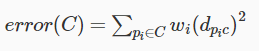
\includegraphics{img/formula_1.png}
\caption{formula\_1}
\end{figure}

where c is the center of the cluster C. The Cluster class includes a
method cluster\_error(data\_table) that takes a Cluster object and the
original data table associated with the counties in the cluster and
computes the error associated with a given cluster.

Given a list of clusters L, the distortion of the clustering is the sum
of the errors associated with its clusters.

\begin{figure}
\centering
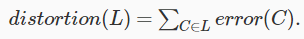
\includegraphics{img/formula_2.png}
\caption{formula\_2}
\end{figure}

    \begin{Verbatim}[commandchars=\\\{\}]
{\color{incolor}In [{\color{incolor}41}]:} \PY{l+s+sd}{\PYZdq{}\PYZdq{}\PYZdq{}}
         \PY{l+s+sd}{compute distortion}
         \PY{l+s+sd}{\PYZdq{}\PYZdq{}\PYZdq{}}
         
         \PY{k+kn}{import} \PY{n+nn}{matplotlib}\PY{n+nn}{.}\PY{n+nn}{pyplot} \PY{k}{as} \PY{n+nn}{plt}
         \PY{k+kn}{import} \PY{n+nn}{csv}
         
         \PY{n}{DATA\PYZus{}TABLE} \PY{o}{=} \PY{p}{[}\PY{p}{]}
         \PY{n}{DATA\PYZus{}URL} \PY{o}{=} \PY{p}{[}\PY{l+s+s1}{\PYZsq{}}\PY{l+s+s1}{unifiedCancerData\PYZus{}111.csv}\PY{l+s+s1}{\PYZsq{}}\PY{p}{,}
                     \PY{l+s+s1}{\PYZsq{}}\PY{l+s+s1}{unifiedCancerData\PYZus{}290.csv}\PY{l+s+s1}{\PYZsq{}}\PY{p}{,}
                     \PY{l+s+s1}{\PYZsq{}}\PY{l+s+s1}{unifiedCancerData\PYZus{}896.csv}\PY{l+s+s1}{\PYZsq{}}\PY{p}{]}
         
         \PY{k}{for} \PY{n}{index} \PY{o+ow}{in} \PY{n+nb}{range}\PY{p}{(}\PY{l+m+mi}{3}\PY{p}{)}\PY{p}{:}
             \PY{k}{with} \PY{n+nb}{open}\PY{p}{(}\PY{n}{DATA\PYZus{}URL}\PY{p}{[}\PY{n}{index}\PY{p}{]}\PY{p}{)} \PY{k}{as} \PY{n}{datafile}\PY{p}{:}
                 \PY{n}{database} \PY{o}{=} \PY{n}{csv}\PY{o}{.}\PY{n}{reader}\PY{p}{(}\PY{n}{datafile}\PY{p}{)}
                 \PY{n}{data\PYZus{}table} \PY{o}{=} \PY{p}{[}\PY{p}{]}
                 \PY{k}{for} \PY{n}{row} \PY{o+ow}{in} \PY{n}{database}\PY{p}{:}
                     \PY{n}{data\PYZus{}table}\PY{o}{.}\PY{n}{append}\PY{p}{(}\PY{p}{[}\PY{n}{row}\PY{p}{[}\PY{l+m+mi}{0}\PY{p}{]}\PY{p}{,} \PY{n+nb}{float}\PY{p}{(}\PY{n}{row}\PY{p}{[}\PY{l+m+mi}{1}\PY{p}{]}\PY{p}{)}\PY{p}{,} \PY{n+nb}{float}\PY{p}{(}\PY{n}{row}\PY{p}{[}\PY{l+m+mi}{2}\PY{p}{]}\PY{p}{)}\PY{p}{,} \PY{n+nb}{int}\PY{p}{(}\PY{n}{row}\PY{p}{[}\PY{l+m+mi}{3}\PY{p}{]}\PY{p}{)}\PY{p}{,} \PY{n+nb}{float}\PY{p}{(}\PY{n}{row}\PY{p}{[}\PY{l+m+mi}{4}\PY{p}{]}\PY{p}{)}\PY{p}{]}\PY{p}{)}
                 \PY{n}{DATA\PYZus{}TABLE}\PY{o}{.}\PY{n}{append}\PY{p}{(}\PY{n}{data\PYZus{}table}\PY{p}{)}
         
         
         \PY{k}{def} \PY{n+nf}{read\PYZus{}data}\PY{p}{(}\PY{n}{data\PYZus{}num}\PY{p}{)}\PY{p}{:}
             \PY{n}{cluster\PYZus{}list} \PY{o}{=} \PY{p}{[}\PY{p}{]}
             \PY{k}{for} \PY{n}{row} \PY{o+ow}{in} \PY{n}{DATA\PYZus{}TABLE}\PY{p}{[}\PY{n}{data\PYZus{}num}\PY{p}{]}\PY{p}{:}
                 \PY{n}{cluster\PYZus{}list}\PY{o}{.}\PY{n}{append}\PY{p}{(}\PY{n}{Cluster}\PY{p}{(}\PY{n+nb}{set}\PY{p}{(}\PY{p}{[}\PY{n}{row}\PY{p}{[}\PY{l+m+mi}{0}\PY{p}{]}\PY{p}{]}\PY{p}{)}\PY{p}{,} \PY{n}{row}\PY{p}{[}\PY{l+m+mi}{1}\PY{p}{]}\PY{p}{,} \PY{n}{row}\PY{p}{[}\PY{l+m+mi}{2}\PY{p}{]}\PY{p}{,} \PY{n}{row}\PY{p}{[}\PY{l+m+mi}{3}\PY{p}{]}\PY{p}{,} \PY{n}{row}\PY{p}{[}\PY{l+m+mi}{4}\PY{p}{]}\PY{p}{)}\PY{p}{)}
         
             \PY{n}{cluster\PYZus{}list}\PY{o}{.}\PY{n}{sort}\PY{p}{(}\PY{n}{key}\PY{o}{=}\PY{k}{lambda} \PY{n}{clstr}\PY{p}{:} \PY{n}{clstr}\PY{o}{.}\PY{n}{horiz\PYZus{}center}\PY{p}{(}\PY{p}{)}\PY{p}{)}
             \PY{k}{return} \PY{n}{cluster\PYZus{}list}
         
         
         \PY{k}{def} \PY{n+nf}{compute\PYZus{}distortion}\PY{p}{(}\PY{n}{cluster\PYZus{}list}\PY{p}{,} \PY{n}{data\PYZus{}table}\PY{p}{)}\PY{p}{:}
             \PY{n}{distortion} \PY{o}{=} \PY{l+m+mi}{0}
             \PY{k}{for} \PY{n}{cluster} \PY{o+ow}{in} \PY{n}{cluster\PYZus{}list}\PY{p}{:}
                 \PY{n}{distortion} \PY{o}{+}\PY{o}{=} \PY{n}{cluster}\PY{o}{.}\PY{n}{cluster\PYZus{}error}\PY{p}{(}\PY{n}{data\PYZus{}table}\PY{p}{)}
             \PY{k}{return} \PY{n}{distortion}
         
         \PY{k}{def} \PY{n+nf}{run\PYZus{}example}\PY{p}{(}\PY{p}{)}\PY{p}{:}
             \PY{n}{cluster\PYZus{}lists} \PY{o}{=} \PY{p}{[}\PY{p}{]}
             \PY{k}{for} \PY{n}{idx} \PY{o+ow}{in} \PY{n+nb}{range}\PY{p}{(}\PY{l+m+mi}{3}\PY{p}{)}\PY{p}{:}
                 \PY{n}{cluster\PYZus{}lists}\PY{o}{.}\PY{n}{append}\PY{p}{(}\PY{n}{read\PYZus{}data}\PY{p}{(}\PY{n}{idx}\PY{p}{)}\PY{p}{)}
         
                 \PY{c+c1}{\PYZsh{} hierarchical method}
                 \PY{n}{cluster\PYZus{}list\PYZus{}pre} \PY{o}{=} \PY{n}{cluster\PYZus{}lists}\PY{p}{[}\PY{n}{idx}\PY{p}{]}
                 \PY{n}{hierarchical\PYZus{}distortion} \PY{o}{=} \PY{p}{[}\PY{p}{]}
                 \PY{k}{for} \PY{n}{num\PYZus{}clusters} \PY{o+ow}{in} \PY{n+nb}{range}\PY{p}{(}\PY{l+m+mi}{20}\PY{p}{,} \PY{l+m+mi}{5}\PY{p}{,} \PY{o}{\PYZhy{}}\PY{l+m+mi}{1}\PY{p}{)}\PY{p}{:}
                     \PY{n}{cluster\PYZus{}list\PYZus{}pre} \PY{o}{=} \PY{n}{hierarchical\PYZus{}clustering}\PY{p}{(}\PY{n}{cluster\PYZus{}list\PYZus{}pre}\PY{p}{,} \PY{n}{num\PYZus{}clusters}\PY{p}{)}
                     \PY{n}{hierarchical\PYZus{}distortion}\PY{o}{.}\PY{n}{append}\PY{p}{(}\PY{n}{compute\PYZus{}distortion}\PY{p}{(}\PY{n}{cluster\PYZus{}list\PYZus{}pre}\PY{p}{,} \PY{n}{DATA\PYZus{}TABLE}\PY{p}{[}\PY{n}{idx}\PY{p}{]}\PY{p}{)}\PY{p}{)}
                 \PY{n}{hierarchical\PYZus{}distortion}\PY{o}{.}\PY{n}{reverse}\PY{p}{(}\PY{p}{)}
         
                 \PY{c+c1}{\PYZsh{} kmeans method}
                 \PY{n}{kmeans\PYZus{}distortion} \PY{o}{=} \PY{p}{[}\PY{p}{]}
                 \PY{k}{for} \PY{n}{num\PYZus{}clusters} \PY{o+ow}{in} \PY{n+nb}{range}\PY{p}{(}\PY{l+m+mi}{6}\PY{p}{,} \PY{l+m+mi}{21}\PY{p}{)}\PY{p}{:}
                     \PY{n}{kmeans\PYZus{}distortion}\PY{o}{.}\PY{n}{append}\PY{p}{(}\PY{n}{compute\PYZus{}distortion}\PY{p}{(}\PY{n}{kmeans\PYZus{}clustering}\PY{p}{(}\PY{n}{cluster\PYZus{}lists}\PY{p}{[}\PY{n}{idx}\PY{p}{]}\PY{p}{,} \PY{n}{num\PYZus{}clusters}\PY{p}{,} \PY{l+m+mi}{5}\PY{p}{)}\PY{p}{,}
                                                                 \PY{n}{DATA\PYZus{}TABLE}\PY{p}{[}\PY{n}{idx}\PY{p}{]}\PY{p}{)}\PY{p}{)}
         
                 \PY{c+c1}{\PYZsh{} plot}
                 \PY{n}{plt}\PY{o}{.}\PY{n}{plot}\PY{p}{(}\PY{n+nb}{list}\PY{p}{(}\PY{n+nb}{range}\PY{p}{(}\PY{l+m+mi}{6}\PY{p}{,} \PY{l+m+mi}{21}\PY{p}{)}\PY{p}{)}\PY{p}{,} \PY{n}{hierarchical\PYZus{}distortion}\PY{p}{,} \PY{l+s+s1}{\PYZsq{}}\PY{l+s+s1}{\PYZhy{}r}\PY{l+s+s1}{\PYZsq{}}\PY{p}{,} \PY{n}{label}\PY{o}{=}\PY{l+s+s1}{\PYZsq{}}\PY{l+s+s1}{hierarchical method}\PY{l+s+s1}{\PYZsq{}}\PY{p}{)}
                 \PY{n}{plt}\PY{o}{.}\PY{n}{plot}\PY{p}{(}\PY{n+nb}{list}\PY{p}{(}\PY{n+nb}{range}\PY{p}{(}\PY{l+m+mi}{6}\PY{p}{,} \PY{l+m+mi}{21}\PY{p}{)}\PY{p}{)}\PY{p}{,} \PY{n}{kmeans\PYZus{}distortion}\PY{p}{,} \PY{l+s+s1}{\PYZsq{}}\PY{l+s+s1}{\PYZhy{}b}\PY{l+s+s1}{\PYZsq{}}\PY{p}{,} \PY{n}{label}\PY{o}{=}\PY{l+s+s1}{\PYZsq{}}\PY{l+s+s1}{kmeans method}\PY{l+s+s1}{\PYZsq{}}\PY{p}{)}
                 \PY{n}{plt}\PY{o}{.}\PY{n}{xlabel}\PY{p}{(}\PY{l+s+s1}{\PYZsq{}}\PY{l+s+s1}{the number of output clusters}\PY{l+s+s1}{\PYZsq{}}\PY{p}{)}
                 \PY{n}{plt}\PY{o}{.}\PY{n}{ylabel}\PY{p}{(}\PY{l+s+s1}{\PYZsq{}}\PY{l+s+s1}{the distortion associated with each output clustering}\PY{l+s+s1}{\PYZsq{}}\PY{p}{)}
                 \PY{n}{plt}\PY{o}{.}\PY{n}{suptitle}\PY{p}{(}\PY{l+s+s1}{\PYZsq{}}\PY{l+s+s1}{the distortion of }\PY{l+s+s1}{\PYZsq{}} \PY{o}{+} \PY{n}{DATA\PYZus{}URL}\PY{p}{[}\PY{n}{idx}\PY{p}{]}\PY{p}{[}\PY{l+m+mi}{18}\PY{p}{:}\PY{l+m+mi}{21}\PY{p}{]} \PY{o}{+} \PY{l+s+s1}{\PYZsq{}}\PY{l+s+s1}{ counties}\PY{l+s+s1}{\PYZsq{}}\PY{p}{)}
                 \PY{n}{plt}\PY{o}{.}\PY{n}{grid}\PY{p}{(}\PY{p}{)}
                 \PY{n}{plt}\PY{o}{.}\PY{n}{legend}\PY{p}{(}\PY{n}{loc}\PY{o}{=}\PY{l+s+s2}{\PYZdq{}}\PY{l+s+s2}{upper right}\PY{l+s+s2}{\PYZdq{}}\PY{p}{)}
                 \PY{n}{plt}\PY{o}{.}\PY{n}{savefig}\PY{p}{(}\PY{n+nb}{str}\PY{p}{(}\PY{n}{idx}\PY{p}{)}\PY{p}{)}
                 \PY{n}{plt}\PY{o}{.}\PY{n}{show}\PY{p}{(}\PY{p}{)}
         
         
         \PY{n}{run\PYZus{}example}\PY{p}{(}\PY{p}{)}
\end{Verbatim}


    \begin{center}
    \adjustimage{max size={0.9\linewidth}{0.9\paperheight}}{output_35_0.png}
    \end{center}
    { \hspace*{\fill} \\}
    
    \begin{center}
    \adjustimage{max size={0.9\linewidth}{0.9\paperheight}}{output_35_1.png}
    \end{center}
    { \hspace*{\fill} \\}
    
    \begin{center}
    \adjustimage{max size={0.9\linewidth}{0.9\paperheight}}{output_35_2.png}
    \end{center}
    { \hspace*{\fill} \\}
    
    So \textbf{only in 111 county data set}, hierarchical method
consistently produce lower distortion, which means hierarchical method
is precise only in 111 data set.

    \section{Conclustion}\label{conclustion}

    For time efficienty: k-means method is O(nm),0\textless{}m\textless{}=n;
hierarchical method is O(n\^{}2*logn). The k-means method is much more
efficient to cluster counties.

However, hierarchical method is more precise to cluster counties than
k-means one when the data is not large.

Therefore, we'd better use hierarchical method when we process data
below 200 sets, and use k-means method to process larger data.


    % Add a bibliography block to the postdoc
    
    
    
    \end{document}
